\chapter{On measuring the fitness of a multiple criteria ranking}
\label{sec:16}

\abstract*{ Starting from a motivating decision problem about how to list, from the best to the worst, a set movies that are star-rated by journalists and movie critics, the chapter shows that \Kendall 's ordinal correlation index tau may be extended to a relational bipolar-valued equivalence measure of  bipolar-valued digraphs. This finding gives way, on the one hand, to measure the fitness and fairness of multiple criteria ranking rules. On the other hand, it provides a tool for illustrating preference divergences between decision objectives and criteria.}

\abstract{ Starting from a motivating decision problem about how to list, from the best to the worst, a set movies that are star-rated by journalists and movie critics, the chapter shows that \Kendall 's ordinal correlation index tau may be extended to a relational bipolar-valued equivalence measure of  bipolar-valued digraphs. This finding gives way, on the one hand, to measure the fitness and fairness of multiple criteria ranking rules. On the other hand, it provides a tool for illustrating preference divergences between decision objectives and criteria.}

\section{Listing movies from best star-rated to worst}
\label{sec:16.1}

In a stubborn keeping with a two-valued logic, where every argument can only be true or false, there is no place for efficiently taking into account missing data or logical indeterminateness. These cases are seen as problematic and, at best are simply ignored. Worst, in modern data science, missing data get often replaced with \emph{fictive} values, potentially falsifying hence all subsequent computations.

In social choice problems, voting abstentions are, however, frequently observed and represent a social expression that may be significant for revealing non represented social preferences. And, in marketing studies, interviewees will not always respond to all the submitted questions. Again, such abstentions do sometimes contain nevertheless valid information concerning consumer preferences.

Such a case is given with  a list of star-rated movies that could be seen in town in September 2003 (source: \emph{Graffiti Star wars}, Edition Revue Luxembourg, September 2007, p. 30.). The underlying performance tableau data, stored in a file named \texttt{graffiti07.py}\footnote{to be found in the \texttt{examples} directory of the \Digraph resources}, is shown below with the \texttt{showHTMLPerformance\-Tableau()} method\index{showHTMLPerformanceTableau@\texttt{showHTMLPerformanceTableau()}}  : 
\begin{lstlisting}
>>> from outrankingDigraphs import\
...                        PerformanceTableau 
>>> gt07 = PerformanceTableau('graffiti07')
>>> gt07.showHTMLPerformanceTableau(\
...               title='Graffiti Star wars',\
...               ndigits=0)
\end{lstlisting}
\begin{figure}[h]
%\sidecaption
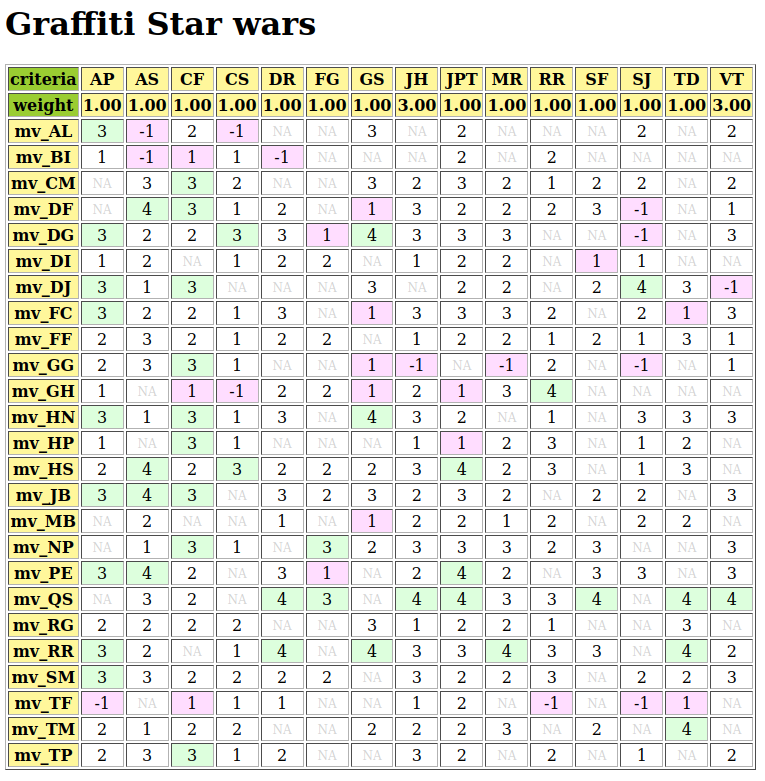
\includegraphics[width=11cm]{Figures/16-1-graffiti07_1.png}
\caption{\emph{Graffiti} magazine's movie ratings from September 2007}
\label{fig:16.1}       % Give a unique label
\end{figure}

Figure~\vref{fig:16.1} shows the star-ratings of $25$ movies by $15$ journalists and movie critics: $5$ stars (\emph{masterpiece}), $4$ stars (\emph{must be seen}), $3$ stars (\emph{excellent}), $2$ stars (\emph{good}), $1$ star (\emph{could be seen}), $-1$ star (\emph{I do not like}), $-2$ stars (\emph{I hate}), \texttt{NA} (\emph{not seen}). Notice in the second row the higher significance ($3.00$) that is granted to two locally renowned movie critics, namely \texttt{JH} and \texttt{VT}. Their opinion counts for three times the opinion of the other critics. With six times a 4 stars (\emph{must be seen}) grade, \texttt{mv\_QS} is best-rated, followed by \texttt{mv\_RR} with four times a 4 stars mark. Fewest stars obtains movie \texttt{mv\_TF} with three times a $-1$ star (\emph{don't like}) mark and five times a $1$ star mark. Notice that many movies, like movie \texttt{mv\_BI}, are only rated by some of the critics. 

To aggregate all the critics' star-ratings, the \emph{Graffiti} magazine computes for each movie a global score --the average weighted number of stars it obtained-- just ignoring the \emph{not seen} movies. Listing~\vref{list:16.1} illustrates below how to compute these global scores using the data stored in the \texttt{gt07} performance tableau. Attribute \texttt{gt07.actions}, resp. \texttt{gt07.criteria}, contains the description of the 25 movies, resp. the 15 critics. The actual star-ratings are to be found in the \texttt{gt07.evaluation} attribute.
\begin{lstlisting}[caption={Computing the average weighted number of stars per movie},label=list:16.1,basicstyle=\ttfamily\scriptsize]
>>> # gt07 = PerformanceTableau('graffiti07')
>>> globalScores = {}
>>> for mv in gt07.actions:
>>>     globalScores[mv] = Decimal('0')
>>>     sumWeights = Decimal('0')
>>>     for critic in gt07.criteria:
>>>         stars = gt07.evaluation[critic][mv]
>>>         if stars != gt07.NA:
>>>             weight = gt07.criteria[critic]['weight']
>>>             globalScores[mv] += (stars * weight)
>>>             sumWeights += weight
>>>     globalScores[mv] /= sumWeights
>>> graffitiList = [(globalScores[mv],mv) for mv in globalScores]
>>> graffitiList.sort(reverse=True)
>>> for item in graffitiList:
>>>     print('%s: %.2f' % (item[1],item[0]) )
  mv_QS: 3.60
  mv_RR: 2.88
  mv_PE: 2.67
  mv_JB: 2.62
  mv_HN: 2.62
  mv_NP: 2.60
  mv_HS: 2.60
  mv_DG: 2.56
  mv_SM: 2.53
  mv_FC: 2.41
  mv_TP: 2.21
  mv_CM: 2.20
  mv_TM: 2.17
  mv_DF: 1.94
  mv_RG: 1.83
  mv_MB: 1.73
  mv_GH: 1.67
  mv_DJ: 1.67
  mv_FF: 1.61
  mv_AL: 1.60
  mv_HP: 1.55
  mv_DI: 1.42
  mv_GG: 0.71
  mv_BI: 0.71
  mv_TF: 0.55
\end{lstlisting}

The global scrores ranking confirms in Lines 17-18 both leading movies --\texttt{mv\_QS} ($3.60$) and \texttt{mv\_RR} ($2.88$) -- as well as in Line 41 the weakest rated one --\texttt{mv\_TF} ($0.55$). Mind however that these global averages, due to the numerous missing grades, are not computed with commensurable denominators; some critics do indeed use a more or less extended range of stars. The movies not seen for instance by critic \texttt{SJ} are favoured, as this critic is severer than others in her rating. Dropping the movies that were not graded by all the critics is not possible either, as none of the $25$ movies was actually rated by all the $15$ critics. Providing a fictive value for the many not seen situations, will as well always somehow falsify the global scores. What to do?

A better approach is to rank the movies on the basis of pairwise bipolar-valued  ``\emph{rated at least as well as}'' statements. Under this epistemic argumentation approach, missing grades are naturally treated as opinion abstentions and hence do not falsify the logical computations. Such a \NetFlows ranking from best-rated to weakest-rated is provided by the \textbf{heatmap} browser view generated with the \texttt{showHTMLPerformanceHeatmap()} method\index{showHTMLPerformanceHeatmap@\texttt{showHTMLPerformanceHeatmap()}} (see List.~\vref{list:16.2}).
\begin{lstlisting}[caption={Showing the movie from best to worst rated in a heatmap view},label=list:16.2]
>>> gt07.showHTMLPerformanceHeatmap(\
...            pageTitle='Ranking the movies',\  
...            rankingRule='NetFlows',
...            Correlations=True,\
...            ndigits=0)
\end{lstlisting}
\begin{figure}[h]
%\sidecaption
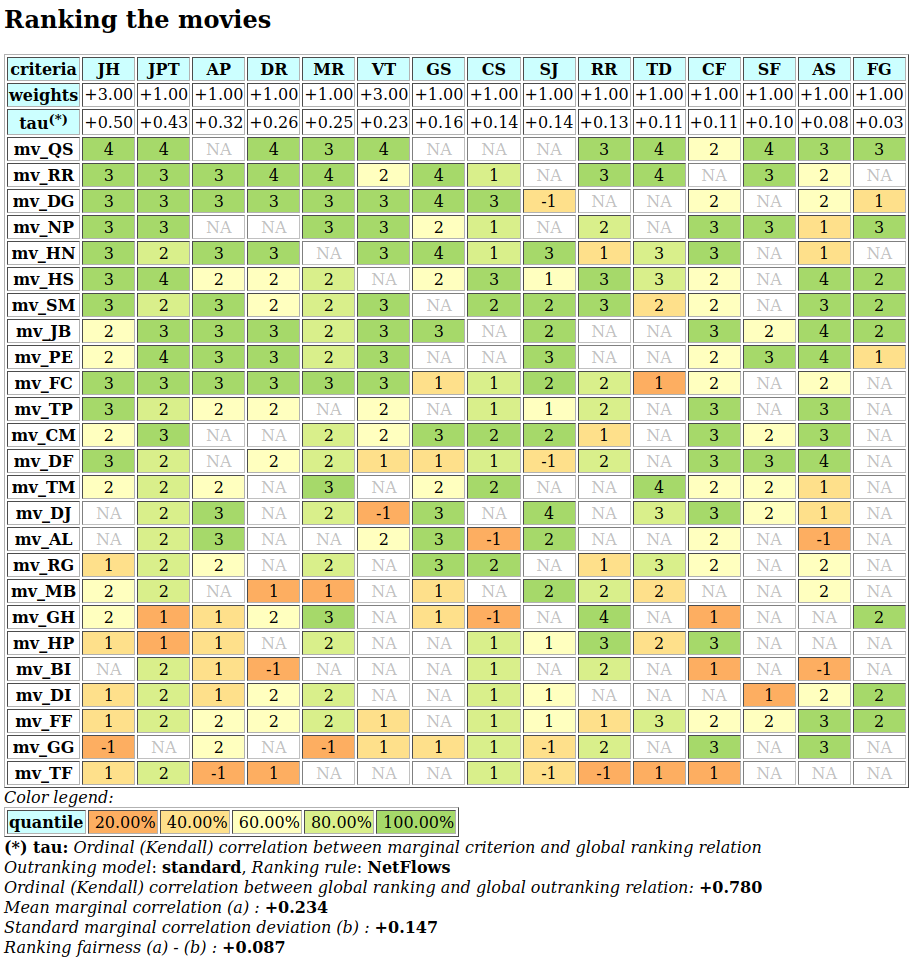
\includegraphics[width=11cm]{Figures/16-2-graffiti07_2.png}
\caption{\emph{Graffiti} magazine's movie ratings from September 2007 ranked with the \NetFlows rule}
\label{fig:16.2}       % Give a unique label
\end{figure}

The \NetFlows ranking shown in Fig.~\vref{fig:16.2} confirms again that movie \texttt{mv\_QS}, with $6$ \emph{must be seen} marks, is correctly best-ranked and the movie \texttt{mv\_TF} is worst-ranked with five \emph{don't like} marks. 

It is fair, however, to eventually mention here that the \emph{Graffiti} magazine's average stars ranking rule is actually showing a very similar result. Indeed, average scores usually confirm well all evident pairwise comparisons, yet \emph{enforce} comparability for all less evident ones. How to judge now the fitness of a given ranking rule?

This is the purpose of the ordinal correlation \emph{tau} indexes shown in Fig.~\vref{fig:16.2} 3rd row. Computing these ordinal correlation indexes is the subject of the next Section.
 
\section{\Kendall 's ordinal correlation tau index}
\label{sec:16:2}

M. G. Kendall\index{Kendall@\emph{Kendall M.G.}} defined his ordinal correlation $\tau$ (\emph{tau}) index for linear orders of dimension $n$ as a balancing of the number $Co$ of correctly oriented pairs against the number $In$ of incorrectly oriented pairs \citep{KEN-1938}. The total number of irreflexive pairs being $n(n-1)$, in the case of linear orders, $Co + In \;=\; n(n-1)$.  Hence $\tau \;=\; \big(\frac{Co}{n(n-1)}\big) \,-\, \big(\frac{In}{n(n-1)}\big)$. In case $In$ is zero, $\tau \;=\; +1$  (all pairs are equivalently oriented); inversely, in case $Co$ is zero, $\tau \;=\; -1$ (all pairs are differently oriented).

Noticing that $\frac{Co}{n(n-1)} \;=\; 1 \,-\, \frac{In}{n(n-1)}$, and recalling that the bipolar-valued negation is operated by changing the sign of the characteristic value:
\begin{equation}
      \tau \;=\; 1 -2\frac{In}{n(n-1)} \;=\; -\big(\,2\frac{In}{n(n-1)} \,-\, 1\,\big) \;=\; 2\frac{Co}{n(n-1)} \,-\, 1,
\end{equation} 
\Kendall 's original \emph{tau} definition implemented in fact the bipolar-valued negation of the non equivalence of two linear orders, i.e. the normalized majority margin of equivalently oriented irreflexive pairs.

Let \texttt{r1} and \texttt{r2} be two random crisp relations defined on a same set of 5 alternatives. We may compute \Kendall 's \emph{tau} index as shown in List.~\vref{list:16.3}.
\begin{lstlisting}[caption={Computing a relational equivalence digraph},label=list:16.3]
>>> from randomDigraphs import RandomDigraph
>>> r1 = RandomDigraph(order=5,Bipolar=True)
>>> r2 = RandomDigraph(order=5,Bipolar=True)
>>> from digraphs import EquivalenceDigraph
>>> eqd = EquivalenceDigraph(r1,r2)
>>> eqd.showRelationTable(ReflexiveTerms=False)
  * ---- Relation Table -----
  r(<=>)|  'a1'	  'a2'	  'a3'	  'a4'	  'a5'	  
  ------|-------------------------------------
   'a1' |    -   -1.00   1.00   -1.00    1.00	 
   'a2' |  -1.00   -    -1.00    1.00   -1.00	 
   'a3' |  -1.00 -1.00    -      1.00    1.00	 
   'a4' |  -1.00  1.00  -1.00     -      1.00	 
   'a5' |  -1.00  1.00  -1.00    1.00     - 	 
   Valuation domain: [-1.00;1.00]
>>> eqd.correlation
  {'correlation': -0.1, 'determination': 1.0}
\end{lstlisting}
In the table of the equivalence relation $(\mathtt{r1}\, \Leftrightarrow\, \mathtt{r2})$ above (see List.~\vref{list:16.1} Lines 10-14), we observe that the normalized majority margin of equivalent versus non equivalent irreflexive pairs amounts to $(9 - 11)/20 = -0.1$, i.e. the value of \Kendall 's \emph{tau} index in this plainly determined crisp case (see Line 17).

What happens now with more or less determined and even partially indeterminate relations? May we proceed in a similar way?

\section{Bipolar-valued relational equivalence}
\label{sec:16.3}

Two random bipolar-valued digraphs \texttt{d1} and \texttt{d2} of order five, generated in List.~\vref{list:16.4}, will help exploring this idea.
\begin{lstlisting}[caption={Two random bipolar-valued digraphs},label=list:16.4]
>>> from randomDigraphs import RandomValuationDigraph
>>> d1 = RandomValuationDigraph(order=5,seed=1)
>>> d1.showRelationTable(ReflexiveTerms=False)
  * ---- Relation Table -----
   r(d1)|   'a1'   'a2'   'a3'   'a4'   'a5'	  
  ------|------------------------------------
   'a1' |    - 	  -0.66	  0.44	  0.94	-0.84	 
   'a2' |  -0.36    - 	 -0.70	  0.26	 0.94	 
   'a3' |   0.14   0.20	   - 	  0.66	-0.04	 
   'a4' |  -0.48 - 0.76	  0.24	   -  	-0.94	 
   'a5' |  -0.02   0.10	  0.54	  0.94    - 	 
   Valuation domain: [-1.00;1.00]
>>> d2 = RandomValuationDigraph(order=5,seed=2)
>>> d2.showRelationTable(ReflexiveTerms=False)
  * ---- Relation Table -----
   r(d2)|   'a1'   'a2'   'a3'   'a4'   'a5'	  
  ------|-----------------------------------
   'a1' |   -     -0.86  -0.78  -0.80  -0.08	 
   'a2' |  -0.58    -     0.88   0.70  -0.22	 
   'a3' |  -0.36   0.54    -    -0.46   0.54	 
   'a4' |  -0.92   0.48   0.74    -    -0.60	 
   'a5' |   0.10   0.62   0.00   0.84    - 	 
   Valuation domain: [-1.00;1.00]
\end{lstlisting}
In the generated random digraphs \texttt{d1} and \texttt{d2}, 9 pairs, like \texttt{(a1,a2)} or \texttt{(a3,a2)} for instance, appear equivalently oriented (see Lines 7,18 or 9,20). The \texttt{Equiva\-lenceDigraph} class\index{EquivalenceDigraph@\texttt{EquivalenceDigraph} class} computes this bipolar-valued relational equivalence between digraphs \texttt{d1} and \texttt{d2} (see List.~\vref{list:16.5}).
\begin{lstlisting}[caption={Bipolar-valued Equivalence Digraph},label=list:16.5]
>>> from digraphs import EquivalenceDigraph
>>> eqd = EquivalenceDigraph(d1,d2)
>>> eqd.showRelationTable(ReflexiveTerms=False)
  * ---- Relation Table -----
   r(<=>)|  'a1'  'a2'   'a3'   'a4'   'a5'	  
   ------|---------------------------------
   'a1' |   - 	  0.66  -0.44  -0.80   0.08	 
    'a2' |  0.36   -    -0.70   0.26  -0.22	 
    'a3' | -0.14  0.20    -    -0.46  -0.04	 
    'a4' |  0.48 -0.48   0.24    -     0.60	 
    'a5' | -0.02  0.10   0.00   0.84    - 	 
   Valuation domain: [-1.00;1.00]
\end{lstlisting}

In our bipolar-valued epistemic logic, logical disjunctions and conjunctions are implemented as $\max$, respectively $\min$ operations. Notice also that the logical equivalence $(\mathtt{d1}\, \Leftrightarrow\, \mathtt{d2})$ corresponds to a double implication $(\mathtt{d1}\, \Rightarrow\, \mathtt{d2})\; \wedge \; (\mathtt{d2}\, \Rightarrow\,  \mathtt{d1})$ and that the implication $(\mathtt{d1} \Rightarrow \mathtt{d2})$ is logically equivalent to the disjunction $(\neg \mathtt{d1} \vee \mathtt{d2})$.

When $r(x\,\mathtt{d1}\, y)$ and $r(x\,\mathtt{d2}\; y)$ denote the bipolar-valued characteristic values of relation \texttt{d1}, resp. \texttt{d2}, we may hence compute as follows a majority margin $M(\mathtt{d1} \Leftrightarrow \mathtt{d2})$ between equivalently and not equivalently oriented irreflexive pairs $(x,y)$:
\begin{equation}\label{eq:16:2}
  \begin{split}
&M(\mathtt{d1} \Leftrightarrow \mathtt{d2}) \; =\\
&\quad \quad \sum_{(x \neq y)} \Big[ \min \Big( \max \big( -r(x \,\mathtt{d1}\, y), r(x \,\mathtt{d2}\, y)\big), \max \big( -r(x \,\mathtt{d2}\, y), r(x \,\mathtt{d1}\, y)\big) \Big) \Big]\;.
\end{split}
\end{equation}

$M(\mathtt{d1} \Leftrightarrow \mathtt{d2})$ is thus given by the sum of the non reflexive terms of the relation table of $eqd$, the relational equivalence digraph computed above (see List.~\vref{list:16.5}). In the crisp case, $M(\mathtt{d1}\,\Leftrightarrow\, \mathtt{d2})$  is normalized with the maximum number of possible irreflexive pairs, namely $n(n-1)$. In the extended $r$-valued case, the maximal possible equivalence majority margin $M$ corresponds to the sum $D$ of the conjoint determinations of $(x \,\mathtt{d1}\, y)$ and $(x \,d2\, y)$ (see \citet{BIS-2012a}):
\begin{equation}
  D \;=\; \sum_{x \neq y} \min \Big[ abs\big(r(x \,\mathtt{d1}\, y) \big), abs \big( r(x \,\mathtt{d2}\, y \big)  \Big]\;,
\end{equation}
and we obtain hence in the general $r$ -valued case:
\begin{equation}\label{eq:16.4}
  \tau(\mathtt{d1},\mathtt{d2}) \;=\; \frac{M(\mathtt{d1}\,\Leftrightarrow\, \mathtt{d2})}{D}\;.
\end{equation}

$\tau(\mathtt{d1},\mathtt{d2})$ corresponds so to the classical ordinal correlation index, yet restricted to the conjointly determined parts of the given digraphs $\mathtt{d1}$ and $\mathtt{d2}$. In the limit case of two crisp linear orders, $D$ equals $n(n-1)$, i.e. the number of irreflexive pairs, and we recover \Kendall 's original \emph{tau} index definition.

It is worthwhile noticing that the ordinal correlation index $\tau(\mathtt{d1},\mathtt{d2})$ one obtains above corresponds in fact to the ratio of:
\begin{itemize}
\item $r(\mathtt{d1}\,\Leftrightarrow\, \mathtt{d2}) \;=\; \frac{M(\mathtt{d1}\,\Leftrightarrow\, \mathtt{d2})}{n(n-1)}$:\\the normalized majority margin of the pairwise \emph{relational} equivalence statements, also called \emph{valued ordinal correlation}, and 
\item $d \;=\; \frac{D}{n(n-1)}$:\\ the normalized determination of the corresponding pairwise relational equivalence statements, in fact the \emph{determinateness} of the relational equivalence digraph.
\end{itemize}

The epistemic determination effect is thus successfully \emph{out-factored} from the ordinal correlation effect. With completely determined relations, $\tau(\mathtt{d1},\mathtt{d2}) \;=\; r(\mathtt{d1}\,\Leftrightarrow\, \mathtt{d2})$. The ordinal correlation with a completely indeterminate digraph, i.e. when $D = 0$, is set by convention to the indeterminate correlation value $0.0$. With uniformly chosen random $r$-valued digraphs, the expected $\tau$ index is $0.0$, denoting in fact an indeterminate relational equivalence. The corresponding expected normalized determination $d$ is about $0.333$ (see \citep{BIS-2012a}).

We may below verify Eq.~\vref{eq:6.4} with help of the equivalence digraph $eqd$ computed in List.~\vref{list:16.5}.
\begin{lstlisting}[caption={Computing the ordinal correlation index from the equivalence digraph},label=list:16.6]
>>> # eqd = EquivalenceDigraph(d1,d2)
>>> M = Decimal('0'); D = Decimal('0')
>>> n2 = eqd.order*(eqd.order - 1)
>>> for x in eqd.actions:
...     for y in eqd.actions:
...         M += eqd.relation[x][y]
...         D += abs(eqd.relation[x][y])
>>> print('r(rd1<=>rd2) = %+.3f, d = %.3f, tau = %+.3f' %\
          (M/n2,D/n2,M/D))   
  r(rd1<=>rd2) = +0.026, d = 0.356, tau = +0.073  
\end{lstlisting}

The \Digraph resources directly provide for the preceding computations the \texttt{compute\-OrdinalCorrelation()} method\index{computeOrdinalCorrelation@\texttt{computeOrdinalCorrelation()}} which renders a dictionary with a \texttt{correlation} ($\tau$) and a \texttt{determina\-tion} ($d$) attribute. We may recover $r(d1\,\Leftrightarrow\, d2)$ by multiplying $\tau$ with $d$ (see List.~\vref{list:16.7} Line 4). 
\begin{lstlisting}[caption={Computing the valued ordinal correlation index},label=list:16.7]
>>> corrd1d2 = d1.computeOrdinalCorrelation(d2)
>>> tau = corrd1d2['correlation']
>>> d = corrd1d2['determination']
>>> r = tau * d
>>> print('tau(d1,d2) = %+.3f, d = %.3f,\
...        r(d1<=>d2) = %+.3f' % (tau, d, r))
  tau(d1,d2) = +0.073, d = 0.356, r(d1<=>d2) = +0.026
\end{lstlisting}

The \Digraph resources provide for convenience a direct \texttt{showCorrela\-tion()} method\index{showCorrelation@\texttt{showCorrelation()}}:
\begin{lstlisting}
>>> d1.showCorrelation(\
...       d1.computeOrdinalCorrelation(d2) )
  Correlation indexes:
    Extended Kendall tau       : +0.073
    Epistemic determination    :  0.356
    Bipolar-valued equivalence : +0.026
\end{lstlisting}

We are now ready for assessing the quality of the \NetFlows ranking of the movies shown in the heat map view of Fig.~\vref{fig:16.2}. 

\section{Fitness of ranking heuristics}
\label{sec:16.3}

The \NetFlows ranking of the movies shown in the heatmap view in Fig.~\vref{fig:16.2} is based on the bipolar-valued outranking digraph modelling the pairwise global ``\emph{rated at least as well as}'' relation among the $25$ movies from the performance tableau instance \texttt{gt07}.
\begin{lstlisting}[caption={The bipolar-valued outranking digraph of the star-rated movies},label=list:16.8]
>>> bod = BipolarOutrankingDigraph(gt07)
  *------- Object instance description ------*
   Instance class   : BipolarOutrankingDigraph
   Instance name    : rel_grafittiPerfTab.xml
   Actions          : 25
   Criteria         : 15
   Size             : 390
   Determinateness  : 65%
   Valuation domain : {'min': Decimal('-1.0'),
                       'med': Decimal('0.0'),
                       'max': Decimal('1.0'),}
>>> g.computeCoSize()
  188
\end{lstlisting}
Listing~\vref{list:16.8} reveals that the outranking digraph \texttt{bod} contains $390$ positively validated (Line 7), $188$ positively invalidated (Line 13)\index{computeCoSize@\texttt{computeCoSize()}}, and 22 indeterminate outranking situations from the potential $25 \times 24 = 600$ irreflexive movie pairs.

Listing~\vref{list:16.9} illustrates with the \texttt{NetFlowsOrder} class \index{NetFlowsOrder@\texttt{NetFlowsOrder} class} from the \texttt{linearOr\-ders} module\index{linearOrders@\texttt{linearOrders} module} how to compute the global \NetFlows ranking \texttt{nf}, as shown in the ordered heat map of Fig.~\vref{fig:16.2} and the bipolar-valued relational equivalence of the \texttt{nf} ranking with each one the individual critic's star-ratings.
\begin{lstlisting}[caption={Computing marginal criterion correlations with global \NetFlows ranking},label=list:16.9]
>>> from linearOrders import NetFlowsOrder
>>> nf = NetFlowsOrder(bod)
>>> nf.netFlowsRanking
  ['mv_QS', 'mv_RR', 'mv_DG', 'mv_NP', 'mv_HN', 'mv_HS', 'mv_SM',
   'mv_JB', 'mv_PE', 'mv_FC', 'mv_TP', 'mv_CM', 'mv_DF', 'mv_TM',
   'mv_DJ', 'mv_AL', 'mv_RG', 'mv_MB', 'mv_GH', 'mv_HP', 'mv_BI',
   'mv_DI', 'mv_FF', 'mv_GG', 'mv_TF']
>>> for i,item in enumerate(\
...       bod.computeMarginalVersusGlobalRankingCorrelations(\
...              nf.netFlowsRanking,ValuedCorrelation=True) ):\
...     print('r(%s<=>nf) = %+.3f' % (item[1],item[0]) )   

  r(JH<=>nf)  = +0.500
  r(JPT<=>nf) = +0.430
  r(AP<=>nf)  = +0.323
  r(DR<=>nf)  = +0.263
  r(MR<=>nf)  = +0.247
  r(VT<=>nf)  = +0.227
  r(GS<=>nf)  = +0.160
  r(CS<=>nf)  = +0.140
  r(SJ<=>nf)  = +0.137
  r(RR<=>nf)  = +0.133
  r(TD<=>nf)  = +0.110
  r(CF<=>nf)  = +0.110
  r(SF<=>nf)  = +0.103
  r(AS<=>nf)  = +0.080
  r(FG<=>nf)  = +0.027
\end{lstlisting}

In List.~\vref{list:16.9} (see Lines 13-27), we obtain the relational equivalence characteristic values shown in the third row of the ranked heatmap (see Fig.~\vref{fig:16.2}). The global \NetFlows ranking \texttt{nf} represents obviously a rather balanced compromise with respect to each movie critic's star-ratings, as there appears no negative correlation with anyone of them. The ranking \texttt{nf} apparently takes also correctly in account that the journalist $JH$, a locally renowned movie critic, shows a higher significance weight (see Line 13).

The ordinal correlation between the global \NetFlows ranking and the outranking digraph \texttt{bod} may be furthermore computed as illstrated in List.~\vref{list:16.10}: 
\begin{lstlisting}[caption={Computing the ordinal correlation between \NetFlows and global outranking digraph},label=list:16.10]
>>> corrgnf = bod.computeOrdinalCorrelation(nf)
>>> bod.showCorrelation(corrgnf)
  Correlation indexes:
    Extended Kendall tau       : +0.780
    Epistemic determination    :  0.300
    Bipolar-valued equivalence : +0.234
\end{lstlisting}
One may notice in Line 4 that the ordinal correlation $\tau(\mathtt{bod},\mathtt{nf})$ index between the \NetFlows ranking $\mathtt{nf}$ and the determined part of the outranking digraph $\mathtt{bod}$ is quite high ($+0.78$). Due to the rather high number of missing data, the $r$ -valued relational equivalence between the $\mathtt{nf}$ and the $\mathtt{bod}$ digraph, with a characteristics value of only $+0.234$, may be misleading. Yet, $+0.234$ still corresponds to a $62\%$ majority support of the movie critics' star-ratings.

It would be interesting to compare similarly the correlations one may obtain with other global ranking heuristics, like the \Copeland ranking rule.

\section{Illustrating preference divergences}
\label{sec:16.4}

The bipolar-valued relational equivalence indexes gives us, via the \texttt{showCrite\-riaCorrelationTable(ValuedCorrelation=True)} method\index{showCriteriaCorrelationTable@\texttt{showCriteriaCorrelationTable()}}, a further measure for studying how \emph{divergent} may appear the rating opinions expressed by the movie critics. 
\begin{figure}[h]
%\sidecaption
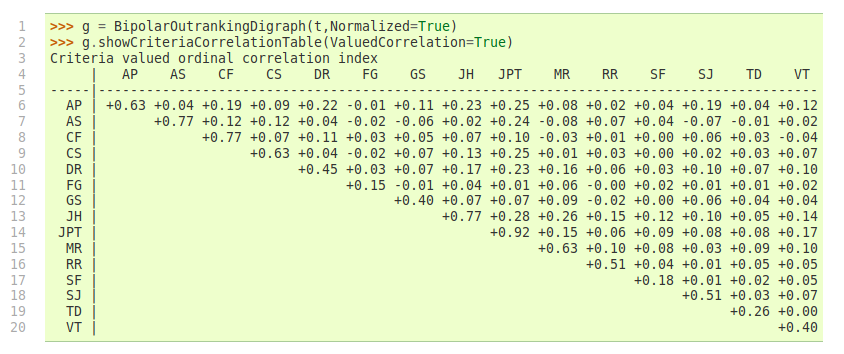
\includegraphics[width=12cm]{Figures/16-3-correlationTable.png}
\caption{Pairwise valued correlation of movie critics.} 
\label{fig:16.3}       % Give a unique label
\end{figure}

It is remarkable to notice in Fig.~\vref{fig:16.3} that, due to the quite numerous missing data, all pairwise valued ordinal correlation indexes $r(x\Leftrightarrow y)$ appear to be of low value, except the diagonal ones. These reflexive indexes $r(x\Leftrightarrow x)$ would trivially all amount to $+1.0$ in a plainly determined case. Here they indicate a reflexive normalized determination score $d$, i.e. the proportion of pairs of movies each critic did evaluate. Critic \texttt{JPT} (the editor of the Graffiti magazine), for instance, evaluated all but one ($d = 24\times23/600 = 0.92$), whereas critic \texttt{FG} evaluated only 10 movies among the 25 in discussion ($d = 10\times9/600 = 0.15$).

To get a picture of the actual divergence of rating opinions concerning jointly seen pairs of movies, we may develop a Principal Component Analysis of the corresponding $\tau$ correlation matrix\footnote{The 3D PCA plot method requires a running R statistics software  (https://www.r-project.org/) installation and the Calmat matrix calculator (see the \texttt{calmat} directory in the \Digraph resources)}. The 3D plot of the first 3 principal axes is shown in Fig.~\vref{fig:16.2}.\index{export3DplotOfCriteriaCorrelation@\texttt{export3DplotOfCriteriaCorrelation()}}
\begin{lstlisting}
>>> bod.export3DplotOfCriteriaCorrelation(\
...                     ValuedCorrelation=False)
\end{lstlisting}
\begin{figure}[h]
%\sidecaption
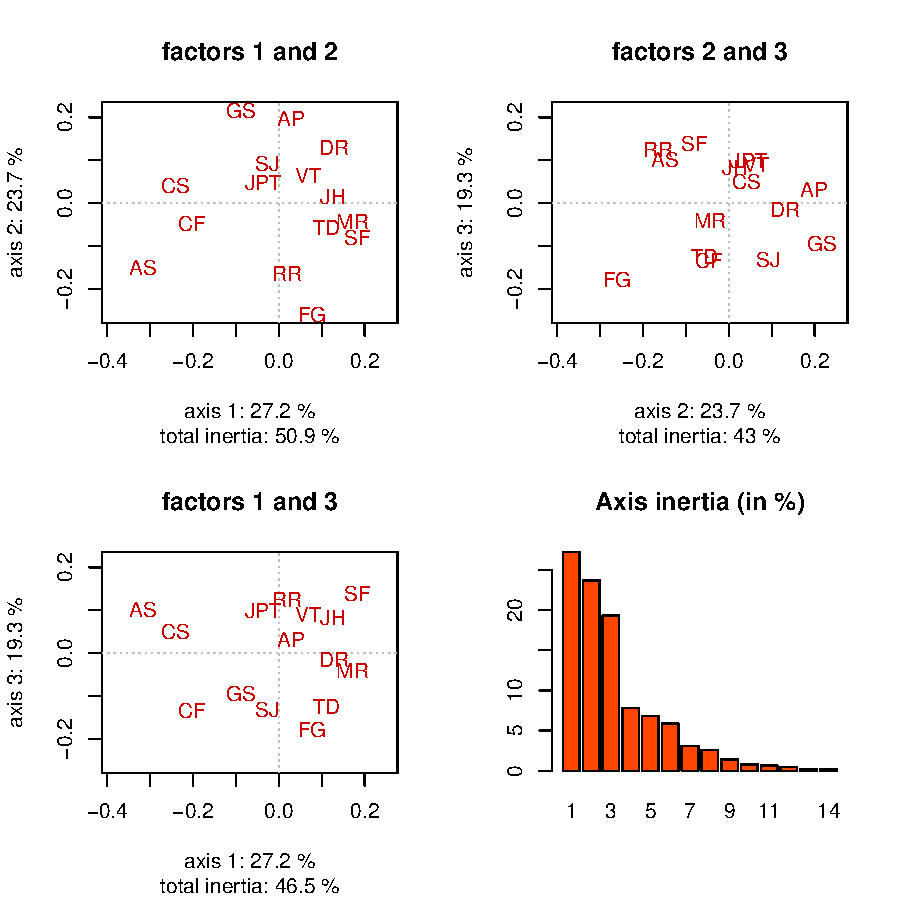
\includegraphics[width=10cm]{Figures/16-4-correlationPCA.pdf}
\caption{3D PCA plot of the criteria ordinal correlation matrix.}
\label{fig:16.4}       % Give a unique label
\end{figure}
The first 3 principal axes support together about $70\%$ of the total inertia. Most eccentric and opposed in their respective rating opinions appear, on the first principal axis with $27.2\%$ inertia, the conservative daily press against labour and public press. On the second principal axis with $23.7.7\%$ inertia, it is the people press versus the cultural critical press. And, on the third axis with still $19.3\%$ inertia, the written media appear most opposed to the radio media.

\section{Exploring the ``\emph{better rated}''  and the ``\emph{as well as rated}'' opinions}
\label{sec:16.5}

In order to furthermore study the quality of a ranking result, it may be interesting to have a separate view on the asymmetric and symmetric parts of the ``\emph{at least as well rated as}'' opinions (see Section \vref{sec:2.3}).

Let us first inspect the pairwise asymmetric part, namely the ``\emph{better rated than}'' and ``\emph{less well rated than}'' opinions of the movie critics. \index{AsymmetricPartialDigraph@\texttt{AsymmetricPartialDigraph} class}
\begin{lstlisting}
>>> from digraphs import AsymmetricPartialDigraph
>>> ag = AsymmetricPartialDigraph(bod)
>>> ag.showHTMLRelationTable(\
...    actionsList=g.computeNetFlowsRanking(),ndigits=0)
\end{lstlisting}
\begin{figure}[h]
%\sidecaption
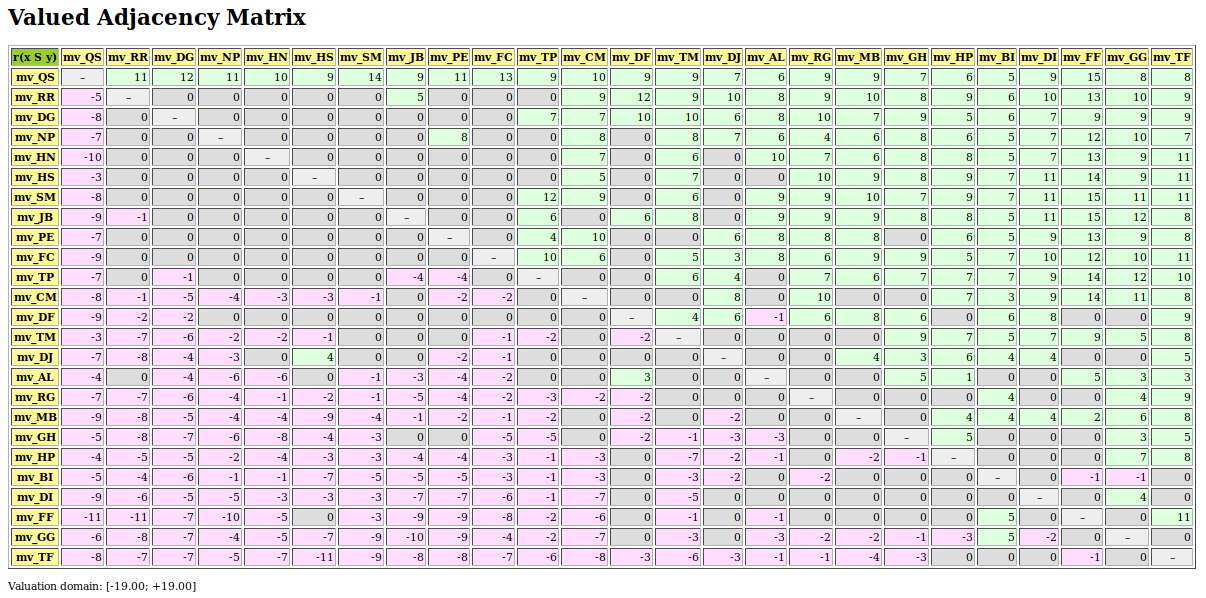
\includegraphics[width=12cm]{Figures/16-5-asymmetricPart.png}
\caption{Asymmetric part of \emph{graffiti07} digraph}
\label{fig:16.5}       % Give a unique label
\end{figure}

We notice in Fig.~\vref{fig:16.5} that the \NetFlows ranking rule inverts in fact just three ``\emph{less well rated than}'' opinions and four ``\emph{better rated than}'' ones. A similar look in Fig.~\vref{fig:16.6} at the symmetric part --the pairwise ``\emph{as well rated as}'' opinions-- suggests a preordered preference structure in several equivalently rated classes. \index{SymmetricPartialDigraph@\texttt{SymmetricPartialDigraph} class}
\begin{lstlisting}
>>> from digraphs import SymmetricPartialDigraph
>>> sg = SymmetricPartialDigraph(bod)
>>> sg.showHTMLRelationTable(\
...          actionsList=g.computeNetFlowsRanking(),\
...          ndigits=0)
\end{lstlisting}
\begin{figure}[h]
%\sidecaption
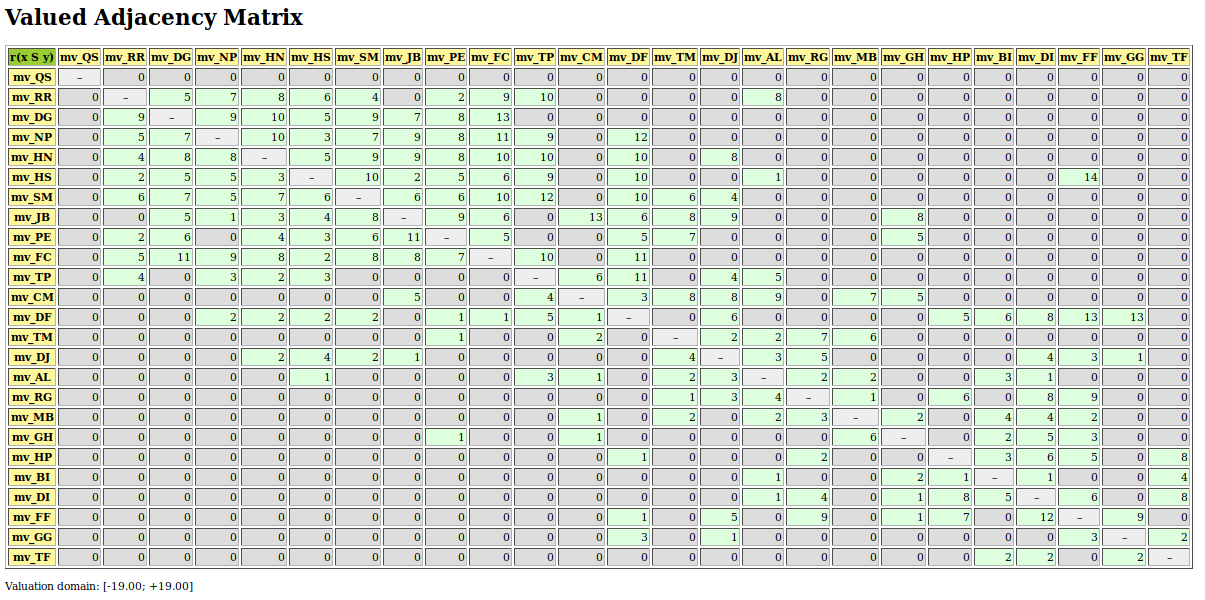
\includegraphics[width=12cm]{Figures/16-6-symmetricPart.png}
\caption{Symmetric part of \emph{graffiti07} digraph}
\label{fig:16.6}       % Give a unique label
\end{figure}

Such a preordering of the movies may, for instance, be computed with the \texttt{compute\-RankingByChoosing()} method\index{computeRankingByChoosing@\texttt{computeRankingByChoosing()}}, where we iteratively extract dominant kernels --best remaining choices-- and absorbent kernels --worst remaining choices-- (see the next Chapter). We operate therefore on the asymmetric ``\emph{better rated than}'' opinions, i.e. the codual of the ``\emph{at least as well rated as}'' opinions \footnote{A kernel in a digraph $g$ is a clique in the dual digraph $-g$.} (see Line 2 in List.~\vref{list:16.11}).
\begin{lstlisting}[caption={Bipolar ranking-by-choosing the Grafitti movies},label=list:16.11]
>>> from transitiveDigraphs import RankingByChoosingDigraph
>>> rbc = RankingByChoosingDigraph(bod,CoDual=True)
>>> rbc.showRankingByChoosing()
  Ranking by Choosing and Rejecting
    1st Best Choice ['mv_QS']
      2nd Best Choice ['mv_DG','mv_FC','mv_HN','mv_HS','mv_NP',
                       'mv_PE','mv_RR','mv_SM']
	3rd Best Choice ['mv_CM','mv_JB','mv_TM']
          4th Best Choice ['mv_AL','mv_TP']
          4th Worst Choice ['mv_AL','mv_TP']
        3rd Worst Choice ['mv_GH','mv_MB','mv_RG']
      2nd Worst Choice ['mv_DF','mv_DJ','mv_FF','mv_GG']
    1st Worst Choice ['mv_BI','mv_DI','mv_HP','mv_TF']
\end{lstlisting}

In the next Chapter~\vref{sec:17}, we thouroughly discuss the computation of such kernels in bipolar-valued digraphs.

%%%%%%% The chapter bibliography
%\normallatexbib
\clearpage
%\phantomsection
%\addcontentsline{toc}{section}{Chapter Bibliography}
\bibliographystyle{spbasic}
%\typeout{}
\bibliography{03-backMatters/reference}
%\chapter{On measuring the fitness of a multiple criteria ranking}
\label{sec:16}

\abstract*{ Starting from a motivating decision problem about how to list, from the best to the worst, a set movies that are star-rated by journalists and movie critics, the chapter shows that \Kendall 's ordinal correlation index tau may be extended to a relational bipolar-valued equivalence measure of  bipolar-valued digraphs. This finding gives way, on the one hand, to measure the fitness and fairness of multiple criteria ranking rules. On the other hand, it provides a tool for illustrating preference divergences between decision objectives and criteria.}

\abstract{ Starting from a motivating decision problem about how to list, from the best to the worst, a set movies that are star-rated by journalists and movie critics, the chapter shows that \Kendall 's ordinal correlation index tau may be extended to a relational bipolar-valued equivalence measure of  bipolar-valued digraphs. This finding gives way, on the one hand, to measure the fitness and fairness of multiple criteria ranking rules. On the other hand, it provides a tool for illustrating preference divergences between decision objectives and criteria.}

\section{Listing movies from best star-rated to worst}
\label{sec:16.1}

In a stubborn keeping with a two-valued logic, where every argument can only be true or false, there is no place for efficiently taking into account missing data or logical indeterminateness. These cases are seen as problematic and, at best are simply ignored. Worst, in modern data science, missing data get often replaced with \emph{fictive} values, potentially falsifying hence all subsequent computations.

In social choice problems, voting abstentions are, however, frequently observed and represent a social expression that may be significant for revealing non represented social preferences. And, in marketing studies, interviewees will not always respond to all the submitted questions. Again, such abstentions do sometimes contain nevertheless valid information concerning consumer preferences.

Such a case is given with  a list of star-rated movies that could be seen in town in September 2003 (source: \emph{Graffiti Star wars}, Edition Revue Luxembourg, September 2007, p. 30.). The underlying performance tableau data, stored in a file named \texttt{graffiti07.py}\footnote{to be found in the \texttt{examples} directory of the \Digraph resources}, is shown below with the \texttt{showHTMLPerformance\-Tableau()} method\index{showHTMLPerformanceTableau@\texttt{showHTMLPerformanceTableau()}}  : 
\begin{lstlisting}
>>> from outrankingDigraphs import\
...                        PerformanceTableau 
>>> gt07 = PerformanceTableau('graffiti07')
>>> gt07.showHTMLPerformanceTableau(\
...               title='Graffiti Star wars',\
...               ndigits=0)
\end{lstlisting}
\begin{figure}[h]
%\sidecaption
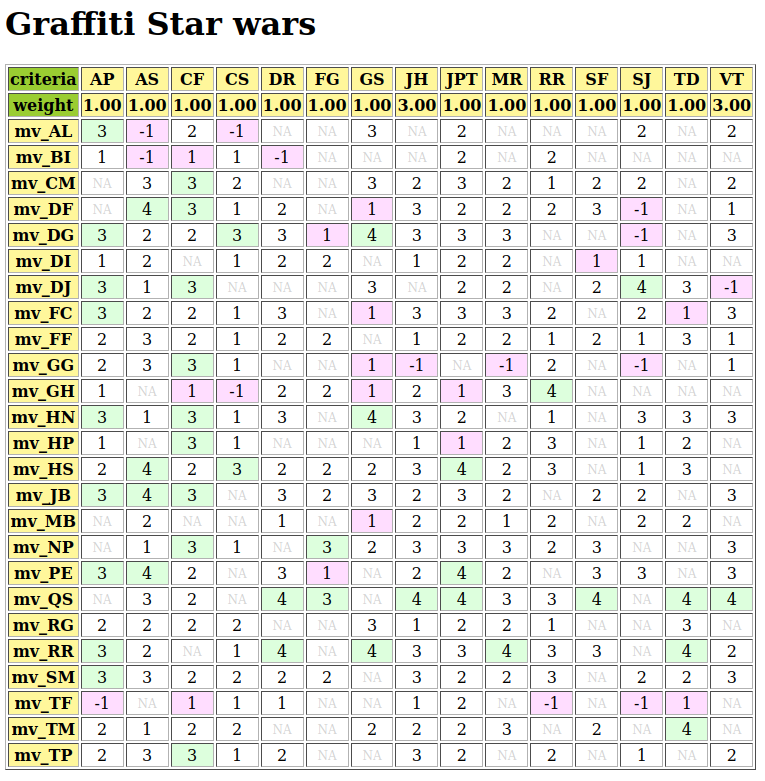
\includegraphics[width=11cm]{Figures/16-1-graffiti07_1.png}
\caption{\emph{Graffiti} magazine's movie ratings from September 2007}
\label{fig:16.1}       % Give a unique label
\end{figure}

Figure~\vref{fig:16.1} shows the star-ratings of $25$ movies by $15$ journalists and movie critics: $5$ stars (\emph{masterpiece}), $4$ stars (\emph{must be seen}), $3$ stars (\emph{excellent}), $2$ stars (\emph{good}), $1$ star (\emph{could be seen}), $-1$ star (\emph{I do not like}), $-2$ stars (\emph{I hate}), \texttt{NA} (\emph{not seen}). Notice in the second row the higher significance ($3.00$) that is granted to two locally renowned movie critics, namely \texttt{JH} and \texttt{VT}. Their opinion counts for three times the opinion of the other critics. With six times a 4 stars (\emph{must be seen}) grade, \texttt{mv\_QS} is best-rated, followed by \texttt{mv\_RR} with four times a 4 stars mark. Fewest stars obtains movie \texttt{mv\_TF} with three times a $-1$ star (\emph{don't like}) mark and five times a $1$ star mark. Notice that many movies, like movie \texttt{mv\_BI}, are only rated by some of the critics. 

To aggregate all the critics' star-ratings, the \emph{Graffiti} magazine computes for each movie a global score --the average weighted number of stars it obtained-- just ignoring the \emph{not seen} movies. Listing~\vref{list:16.1} illustrates below how to compute these global scores using the data stored in the \texttt{gt07} performance tableau. Attribute \texttt{gt07.actions}, resp. \texttt{gt07.criteria}, contains the description of the 25 movies, resp. the 15 critics. The actual star-ratings are to be found in the \texttt{gt07.evaluation} attribute.
\begin{lstlisting}[caption={Computing the average weighted number of stars per movie},label=list:16.1,basicstyle=\ttfamily\scriptsize]
>>> # gt07 = PerformanceTableau('graffiti07')
>>> globalScores = {}
>>> for mv in gt07.actions:
>>>     globalScores[mv] = Decimal('0')
>>>     sumWeights = Decimal('0')
>>>     for critic in gt07.criteria:
>>>         stars = gt07.evaluation[critic][mv]
>>>         if stars != gt07.NA:
>>>             weight = gt07.criteria[critic]['weight']
>>>             globalScores[mv] += (stars * weight)
>>>             sumWeights += weight
>>>     globalScores[mv] /= sumWeights
>>> graffitiList = [(globalScores[mv],mv) for mv in globalScores]
>>> graffitiList.sort(reverse=True)
>>> for item in graffitiList:
>>>     print('%s: %.2f' % (item[1],item[0]) )
  mv_QS: 3.60
  mv_RR: 2.88
  mv_PE: 2.67
  mv_JB: 2.62
  mv_HN: 2.62
  mv_NP: 2.60
  mv_HS: 2.60
  mv_DG: 2.56
  mv_SM: 2.53
  mv_FC: 2.41
  mv_TP: 2.21
  mv_CM: 2.20
  mv_TM: 2.17
  mv_DF: 1.94
  mv_RG: 1.83
  mv_MB: 1.73
  mv_GH: 1.67
  mv_DJ: 1.67
  mv_FF: 1.61
  mv_AL: 1.60
  mv_HP: 1.55
  mv_DI: 1.42
  mv_GG: 0.71
  mv_BI: 0.71
  mv_TF: 0.55
\end{lstlisting}

The global scrores ranking confirms in Lines 17-18 both leading movies --\texttt{mv\_QS} ($3.60$) and \texttt{mv\_RR} ($2.88$) -- as well as in Line 41 the weakest rated one --\texttt{mv\_TF} ($0.55$). Mind however that these global averages, due to the numerous missing grades, are not computed with commensurable denominators; some critics do indeed use a more or less extended range of stars. The movies not seen for instance by critic \texttt{SJ} are favoured, as this critic is severer than others in her rating. Dropping the movies that were not graded by all the critics is not possible either, as none of the $25$ movies was actually rated by all the $15$ critics. Providing a fictive value for the many not seen situations, will as well always somehow falsify the global scores. What to do?

A better approach is to rank the movies on the basis of pairwise bipolar-valued  ``\emph{rated at least as well as}'' statements. Under this epistemic argumentation approach, missing grades are naturally treated as opinion abstentions and hence do not falsify the logical computations. Such a \NetFlows ranking from best-rated to weakest-rated is provided by the \textbf{heatmap} browser view generated with the \texttt{showHTMLPerformanceHeatmap()} method\index{showHTMLPerformanceHeatmap@\texttt{showHTMLPerformanceHeatmap()}} (see List.~\vref{list:16.2}).
\begin{lstlisting}[caption={Showing the movie from best to worst rated in a heatmap view},label=list:16.2]
>>> gt07.showHTMLPerformanceHeatmap(\
...            pageTitle='Ranking the movies',\  
...            rankingRule='NetFlows',
...            Correlations=True,\
...            ndigits=0)
\end{lstlisting}
\begin{figure}[h]
%\sidecaption
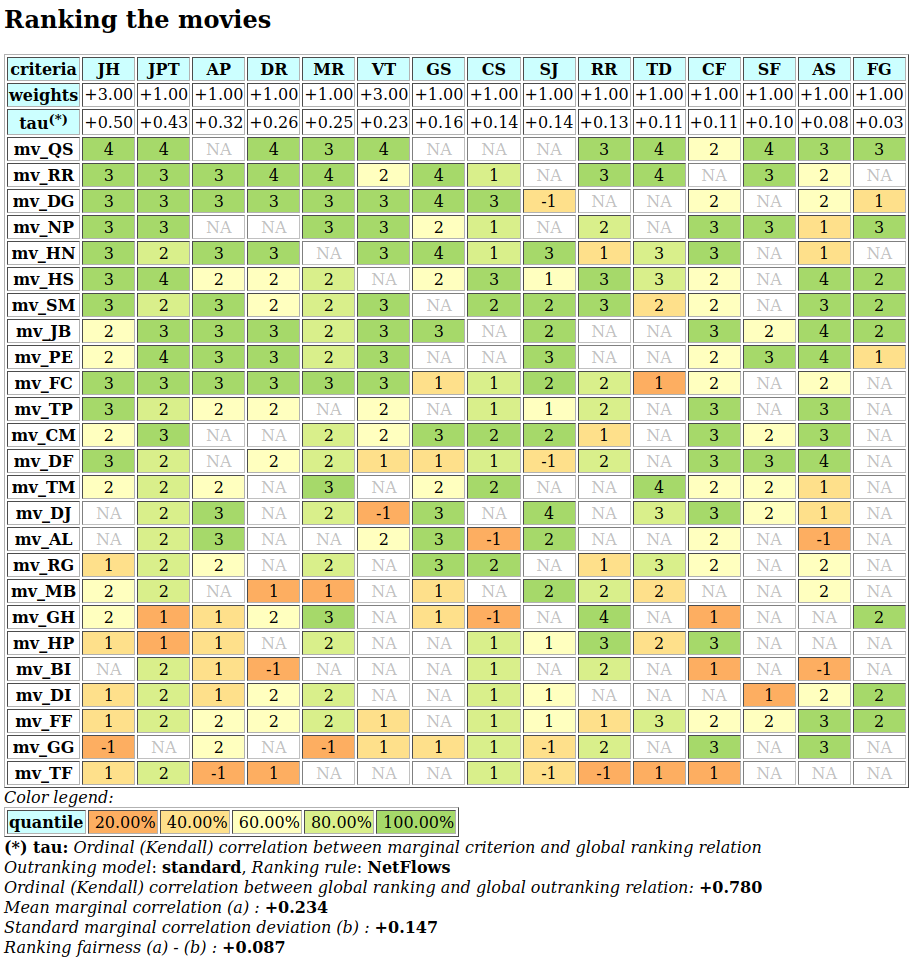
\includegraphics[width=11cm]{Figures/16-2-graffiti07_2.png}
\caption{\emph{Graffiti} magazine's movie ratings from September 2007 ranked with the \NetFlows rule}
\label{fig:16.2}       % Give a unique label
\end{figure}

The \NetFlows ranking shown in Fig.~\vref{fig:16.2} confirms again that movie \texttt{mv\_QS}, with $6$ \emph{must be seen} marks, is correctly best-ranked and the movie \texttt{mv\_TF} is worst-ranked with five \emph{don't like} marks. 

It is fair, however, to eventually mention here that the \emph{Graffiti} magazine's average stars ranking rule is actually showing a very similar result. Indeed, average scores usually confirm well all evident pairwise comparisons, yet \emph{enforce} comparability for all less evident ones. How to judge now the fitness of a given ranking rule?

This is the purpose of the ordinal correlation \emph{tau} indexes shown in Fig.~\vref{fig:16.2} 3rd row. Computing these ordinal correlation indexes is the subject of the next Section.
 
\section{\Kendall 's ordinal correlation tau index}
\label{sec:16:2}

M. G. Kendall\index{Kendall@\emph{Kendall M.G.}} defined his ordinal correlation $\tau$ (\emph{tau}) index for linear orders of dimension $n$ as a balancing of the number $Co$ of correctly oriented pairs against the number $In$ of incorrectly oriented pairs \citep{KEN-1938}. The total number of irreflexive pairs being $n(n-1)$, in the case of linear orders, $Co + In \;=\; n(n-1)$.  Hence $\tau \;=\; \big(\frac{Co}{n(n-1)}\big) \,-\, \big(\frac{In}{n(n-1)}\big)$. In case $In$ is zero, $\tau \;=\; +1$  (all pairs are equivalently oriented); inversely, in case $Co$ is zero, $\tau \;=\; -1$ (all pairs are differently oriented).

Noticing that $\frac{Co}{n(n-1)} \;=\; 1 \,-\, \frac{In}{n(n-1)}$, and recalling that the bipolar-valued negation is operated by changing the sign of the characteristic value:
\begin{equation}
      \tau \;=\; 1 -2\frac{In}{n(n-1)} \;=\; -\big(\,2\frac{In}{n(n-1)} \,-\, 1\,\big) \;=\; 2\frac{Co}{n(n-1)} \,-\, 1,
\end{equation} 
\Kendall 's original \emph{tau} definition implemented in fact the bipolar-valued negation of the non equivalence of two linear orders, i.e. the normalized majority margin of equivalently oriented irreflexive pairs.

Let \texttt{r1} and \texttt{r2} be two random crisp relations defined on a same set of 5 alternatives. We may compute \Kendall 's \emph{tau} index as shown in List.~\vref{list:16.3}.
\begin{lstlisting}[caption={Computing a relational equivalence digraph},label=list:16.3]
>>> from randomDigraphs import RandomDigraph
>>> r1 = RandomDigraph(order=5,Bipolar=True)
>>> r2 = RandomDigraph(order=5,Bipolar=True)
>>> from digraphs import EquivalenceDigraph
>>> eqd = EquivalenceDigraph(r1,r2)
>>> eqd.showRelationTable(ReflexiveTerms=False)
  * ---- Relation Table -----
  r(<=>)|  'a1'	  'a2'	  'a3'	  'a4'	  'a5'	  
  ------|-------------------------------------
   'a1' |    -   -1.00   1.00   -1.00    1.00	 
   'a2' |  -1.00   -    -1.00    1.00   -1.00	 
   'a3' |  -1.00 -1.00    -      1.00    1.00	 
   'a4' |  -1.00  1.00  -1.00     -      1.00	 
   'a5' |  -1.00  1.00  -1.00    1.00     - 	 
   Valuation domain: [-1.00;1.00]
>>> eqd.correlation
  {'correlation': -0.1, 'determination': 1.0}
\end{lstlisting}
In the table of the equivalence relation $(\mathtt{r1}\, \Leftrightarrow\, \mathtt{r2})$ above (see List.~\vref{list:16.1} Lines 10-14), we observe that the normalized majority margin of equivalent versus non equivalent irreflexive pairs amounts to $(9 - 11)/20 = -0.1$, i.e. the value of \Kendall 's \emph{tau} index in this plainly determined crisp case (see Line 17).

What happens now with more or less determined and even partially indeterminate relations? May we proceed in a similar way?

\section{Bipolar-valued relational equivalence}
\label{sec:16.3}

Two random bipolar-valued digraphs \texttt{d1} and \texttt{d2} of order five, generated in List.~\vref{list:16.4}, will help exploring this idea.
\begin{lstlisting}[caption={Two random bipolar-valued digraphs},label=list:16.4]
>>> from randomDigraphs import RandomValuationDigraph
>>> d1 = RandomValuationDigraph(order=5,seed=1)
>>> d1.showRelationTable(ReflexiveTerms=False)
  * ---- Relation Table -----
   r(d1)|   'a1'   'a2'   'a3'   'a4'   'a5'	  
  ------|------------------------------------
   'a1' |    - 	  -0.66	  0.44	  0.94	-0.84	 
   'a2' |  -0.36    - 	 -0.70	  0.26	 0.94	 
   'a3' |   0.14   0.20	   - 	  0.66	-0.04	 
   'a4' |  -0.48 - 0.76	  0.24	   -  	-0.94	 
   'a5' |  -0.02   0.10	  0.54	  0.94    - 	 
   Valuation domain: [-1.00;1.00]
>>> d2 = RandomValuationDigraph(order=5,seed=2)
>>> d2.showRelationTable(ReflexiveTerms=False)
  * ---- Relation Table -----
   r(d2)|   'a1'   'a2'   'a3'   'a4'   'a5'	  
  ------|-----------------------------------
   'a1' |   -     -0.86  -0.78  -0.80  -0.08	 
   'a2' |  -0.58    -     0.88   0.70  -0.22	 
   'a3' |  -0.36   0.54    -    -0.46   0.54	 
   'a4' |  -0.92   0.48   0.74    -    -0.60	 
   'a5' |   0.10   0.62   0.00   0.84    - 	 
   Valuation domain: [-1.00;1.00]
\end{lstlisting}
In the generated random digraphs \texttt{d1} and \texttt{d2}, 9 pairs, like \texttt{(a1,a2)} or \texttt{(a3,a2)} for instance, appear equivalently oriented (see Lines 7,18 or 9,20). The \texttt{Equiva\-lenceDigraph} class\index{EquivalenceDigraph@\texttt{EquivalenceDigraph} class} computes this bipolar-valued relational equivalence between digraphs \texttt{d1} and \texttt{d2} (see List.~\vref{list:16.5}).
\begin{lstlisting}[caption={Bipolar-valued Equivalence Digraph},label=list:16.5]
>>> from digraphs import EquivalenceDigraph
>>> eqd = EquivalenceDigraph(d1,d2)
>>> eqd.showRelationTable(ReflexiveTerms=False)
  * ---- Relation Table -----
   r(<=>)|  'a1'  'a2'   'a3'   'a4'   'a5'	  
   ------|---------------------------------
   'a1' |   - 	  0.66  -0.44  -0.80   0.08	 
    'a2' |  0.36   -    -0.70   0.26  -0.22	 
    'a3' | -0.14  0.20    -    -0.46  -0.04	 
    'a4' |  0.48 -0.48   0.24    -     0.60	 
    'a5' | -0.02  0.10   0.00   0.84    - 	 
   Valuation domain: [-1.00;1.00]
\end{lstlisting}

In our bipolar-valued epistemic logic, logical disjunctions and conjunctions are implemented as $\max$, respectively $\min$ operations. Notice also that the logical equivalence $(\mathtt{d1}\, \Leftrightarrow\, \mathtt{d2})$ corresponds to a double implication $(\mathtt{d1}\, \Rightarrow\, \mathtt{d2})\; \wedge \; (\mathtt{d2}\, \Rightarrow\,  \mathtt{d1})$ and that the implication $(\mathtt{d1} \Rightarrow \mathtt{d2})$ is logically equivalent to the disjunction $(\neg \mathtt{d1} \vee \mathtt{d2})$.

When $r(x\,\mathtt{d1}\, y)$ and $r(x\,\mathtt{d2}\; y)$ denote the bipolar-valued characteristic values of relation \texttt{d1}, resp. \texttt{d2}, we may hence compute as follows a majority margin $M(\mathtt{d1} \Leftrightarrow \mathtt{d2})$ between equivalently and not equivalently oriented irreflexive pairs $(x,y)$:
\begin{equation}\label{eq:16:2}
  \begin{split}
&M(\mathtt{d1} \Leftrightarrow \mathtt{d2}) \; =\\
&\quad \quad \sum_{(x \neq y)} \Big[ \min \Big( \max \big( -r(x \,\mathtt{d1}\, y), r(x \,\mathtt{d2}\, y)\big), \max \big( -r(x \,\mathtt{d2}\, y), r(x \,\mathtt{d1}\, y)\big) \Big) \Big]\;.
\end{split}
\end{equation}

$M(\mathtt{d1} \Leftrightarrow \mathtt{d2})$ is thus given by the sum of the non reflexive terms of the relation table of $eqd$, the relational equivalence digraph computed above (see List.~\vref{list:16.5}). In the crisp case, $M(\mathtt{d1}\,\Leftrightarrow\, \mathtt{d2})$  is normalized with the maximum number of possible irreflexive pairs, namely $n(n-1)$. In the extended $r$-valued case, the maximal possible equivalence majority margin $M$ corresponds to the sum $D$ of the conjoint determinations of $(x \,\mathtt{d1}\, y)$ and $(x \,d2\, y)$ (see \citet{BIS-2012a}):
\begin{equation}
  D \;=\; \sum_{x \neq y} \min \Big[ abs\big(r(x \,\mathtt{d1}\, y) \big), abs \big( r(x \,\mathtt{d2}\, y \big)  \Big]\;,
\end{equation}
and we obtain hence in the general $r$ -valued case:
\begin{equation}\label{eq:16.4}
  \tau(\mathtt{d1},\mathtt{d2}) \;=\; \frac{M(\mathtt{d1}\,\Leftrightarrow\, \mathtt{d2})}{D}\;.
\end{equation}

$\tau(\mathtt{d1},\mathtt{d2})$ corresponds so to the classical ordinal correlation index, yet restricted to the conjointly determined parts of the given digraphs $\mathtt{d1}$ and $\mathtt{d2}$. In the limit case of two crisp linear orders, $D$ equals $n(n-1)$, i.e. the number of irreflexive pairs, and we recover \Kendall 's original \emph{tau} index definition.

It is worthwhile noticing that the ordinal correlation index $\tau(\mathtt{d1},\mathtt{d2})$ one obtains above corresponds in fact to the ratio of:
\begin{itemize}
\item $r(\mathtt{d1}\,\Leftrightarrow\, \mathtt{d2}) \;=\; \frac{M(\mathtt{d1}\,\Leftrightarrow\, \mathtt{d2})}{n(n-1)}$:\\the normalized majority margin of the pairwise \emph{relational} equivalence statements, also called \emph{valued ordinal correlation}, and 
\item $d \;=\; \frac{D}{n(n-1)}$:\\ the normalized determination of the corresponding pairwise relational equivalence statements, in fact the \emph{determinateness} of the relational equivalence digraph.
\end{itemize}

The epistemic determination effect is thus successfully \emph{out-factored} from the ordinal correlation effect. With completely determined relations, $\tau(\mathtt{d1},\mathtt{d2}) \;=\; r(\mathtt{d1}\,\Leftrightarrow\, \mathtt{d2})$. The ordinal correlation with a completely indeterminate digraph, i.e. when $D = 0$, is set by convention to the indeterminate correlation value $0.0$. With uniformly chosen random $r$-valued digraphs, the expected $\tau$ index is $0.0$, denoting in fact an indeterminate relational equivalence. The corresponding expected normalized determination $d$ is about $0.333$ (see \citep{BIS-2012a}).

We may below verify Eq.~\vref{eq:6.4} with help of the equivalence digraph $eqd$ computed in List.~\vref{list:16.5}.
\begin{lstlisting}[caption={Computing the ordinal correlation index from the equivalence digraph},label=list:16.6]
>>> # eqd = EquivalenceDigraph(d1,d2)
>>> M = Decimal('0'); D = Decimal('0')
>>> n2 = eqd.order*(eqd.order - 1)
>>> for x in eqd.actions:
...     for y in eqd.actions:
...         M += eqd.relation[x][y]
...         D += abs(eqd.relation[x][y])
>>> print('r(rd1<=>rd2) = %+.3f, d = %.3f, tau = %+.3f' %\
          (M/n2,D/n2,M/D))   
  r(rd1<=>rd2) = +0.026, d = 0.356, tau = +0.073  
\end{lstlisting}

The \Digraph resources directly provide for the preceding computations the \texttt{compute\-OrdinalCorrelation()} method\index{computeOrdinalCorrelation@\texttt{computeOrdinalCorrelation()}} which renders a dictionary with a \texttt{correlation} ($\tau$) and a \texttt{determina\-tion} ($d$) attribute. We may recover $r(d1\,\Leftrightarrow\, d2)$ by multiplying $\tau$ with $d$ (see List.~\vref{list:16.7} Line 4). 
\begin{lstlisting}[caption={Computing the valued ordinal correlation index},label=list:16.7]
>>> corrd1d2 = d1.computeOrdinalCorrelation(d2)
>>> tau = corrd1d2['correlation']
>>> d = corrd1d2['determination']
>>> r = tau * d
>>> print('tau(d1,d2) = %+.3f, d = %.3f,\
...        r(d1<=>d2) = %+.3f' % (tau, d, r))
  tau(d1,d2) = +0.073, d = 0.356, r(d1<=>d2) = +0.026
\end{lstlisting}

The \Digraph resources provide for convenience a direct \texttt{showCorrela\-tion()} method\index{showCorrelation@\texttt{showCorrelation()}}:
\begin{lstlisting}
>>> d1.showCorrelation(\
...       d1.computeOrdinalCorrelation(d2) )
  Correlation indexes:
    Extended Kendall tau       : +0.073
    Epistemic determination    :  0.356
    Bipolar-valued equivalence : +0.026
\end{lstlisting}

We are now ready for assessing the quality of the \NetFlows ranking of the movies shown in the heat map view of Fig.~\vref{fig:16.2}. 

\section{Fitness of ranking heuristics}
\label{sec:16.3}

The \NetFlows ranking of the movies shown in the heatmap view in Fig.~\vref{fig:16.2} is based on the bipolar-valued outranking digraph modelling the pairwise global ``\emph{rated at least as well as}'' relation among the $25$ movies from the performance tableau instance \texttt{gt07}.
\begin{lstlisting}[caption={The bipolar-valued outranking digraph of the star-rated movies},label=list:16.8]
>>> bod = BipolarOutrankingDigraph(gt07)
  *------- Object instance description ------*
   Instance class   : BipolarOutrankingDigraph
   Instance name    : rel_grafittiPerfTab.xml
   Actions          : 25
   Criteria         : 15
   Size             : 390
   Determinateness  : 65%
   Valuation domain : {'min': Decimal('-1.0'),
                       'med': Decimal('0.0'),
                       'max': Decimal('1.0'),}
>>> g.computeCoSize()
  188
\end{lstlisting}
Listing~\vref{list:16.8} reveals that the outranking digraph \texttt{bod} contains $390$ positively validated (Line 7), $188$ positively invalidated (Line 13)\index{computeCoSize@\texttt{computeCoSize()}}, and 22 indeterminate outranking situations from the potential $25 \times 24 = 600$ irreflexive movie pairs.

Listing~\vref{list:16.9} illustrates with the \texttt{NetFlowsOrder} class \index{NetFlowsOrder@\texttt{NetFlowsOrder} class} from the \texttt{linearOr\-ders} module\index{linearOrders@\texttt{linearOrders} module} how to compute the global \NetFlows ranking \texttt{nf}, as shown in the ordered heat map of Fig.~\vref{fig:16.2} and the bipolar-valued relational equivalence of the \texttt{nf} ranking with each one the individual critic's star-ratings.
\begin{lstlisting}[caption={Computing marginal criterion correlations with global \NetFlows ranking},label=list:16.9]
>>> from linearOrders import NetFlowsOrder
>>> nf = NetFlowsOrder(bod)
>>> nf.netFlowsRanking
  ['mv_QS', 'mv_RR', 'mv_DG', 'mv_NP', 'mv_HN', 'mv_HS', 'mv_SM',
   'mv_JB', 'mv_PE', 'mv_FC', 'mv_TP', 'mv_CM', 'mv_DF', 'mv_TM',
   'mv_DJ', 'mv_AL', 'mv_RG', 'mv_MB', 'mv_GH', 'mv_HP', 'mv_BI',
   'mv_DI', 'mv_FF', 'mv_GG', 'mv_TF']
>>> for i,item in enumerate(\
...       bod.computeMarginalVersusGlobalRankingCorrelations(\
...              nf.netFlowsRanking,ValuedCorrelation=True) ):\
...     print('r(%s<=>nf) = %+.3f' % (item[1],item[0]) )   

  r(JH<=>nf)  = +0.500
  r(JPT<=>nf) = +0.430
  r(AP<=>nf)  = +0.323
  r(DR<=>nf)  = +0.263
  r(MR<=>nf)  = +0.247
  r(VT<=>nf)  = +0.227
  r(GS<=>nf)  = +0.160
  r(CS<=>nf)  = +0.140
  r(SJ<=>nf)  = +0.137
  r(RR<=>nf)  = +0.133
  r(TD<=>nf)  = +0.110
  r(CF<=>nf)  = +0.110
  r(SF<=>nf)  = +0.103
  r(AS<=>nf)  = +0.080
  r(FG<=>nf)  = +0.027
\end{lstlisting}

In List.~\vref{list:16.9} (see Lines 13-27), we obtain the relational equivalence characteristic values shown in the third row of the ranked heatmap (see Fig.~\vref{fig:16.2}). The global \NetFlows ranking \texttt{nf} represents obviously a rather balanced compromise with respect to each movie critic's star-ratings, as there appears no negative correlation with anyone of them. The ranking \texttt{nf} apparently takes also correctly in account that the journalist $JH$, a locally renowned movie critic, shows a higher significance weight (see Line 13).

The ordinal correlation between the global \NetFlows ranking and the outranking digraph \texttt{bod} may be furthermore computed as illstrated in List.~\vref{list:16.10}: 
\begin{lstlisting}[caption={Computing the ordinal correlation between \NetFlows and global outranking digraph},label=list:16.10]
>>> corrgnf = bod.computeOrdinalCorrelation(nf)
>>> bod.showCorrelation(corrgnf)
  Correlation indexes:
    Extended Kendall tau       : +0.780
    Epistemic determination    :  0.300
    Bipolar-valued equivalence : +0.234
\end{lstlisting}
One may notice in Line 4 that the ordinal correlation $\tau(\mathtt{bod},\mathtt{nf})$ index between the \NetFlows ranking $\mathtt{nf}$ and the determined part of the outranking digraph $\mathtt{bod}$ is quite high ($+0.78$). Due to the rather high number of missing data, the $r$ -valued relational equivalence between the $\mathtt{nf}$ and the $\mathtt{bod}$ digraph, with a characteristics value of only $+0.234$, may be misleading. Yet, $+0.234$ still corresponds to a $62\%$ majority support of the movie critics' star-ratings.

It would be interesting to compare similarly the correlations one may obtain with other global ranking heuristics, like the \Copeland ranking rule.

\section{Illustrating preference divergences}
\label{sec:16.4}

The bipolar-valued relational equivalence indexes gives us, via the \texttt{showCrite\-riaCorrelationTable(ValuedCorrelation=True)} method\index{showCriteriaCorrelationTable@\texttt{showCriteriaCorrelationTable()}}, a further measure for studying how \emph{divergent} may appear the rating opinions expressed by the movie critics. 
\begin{figure}[h]
%\sidecaption
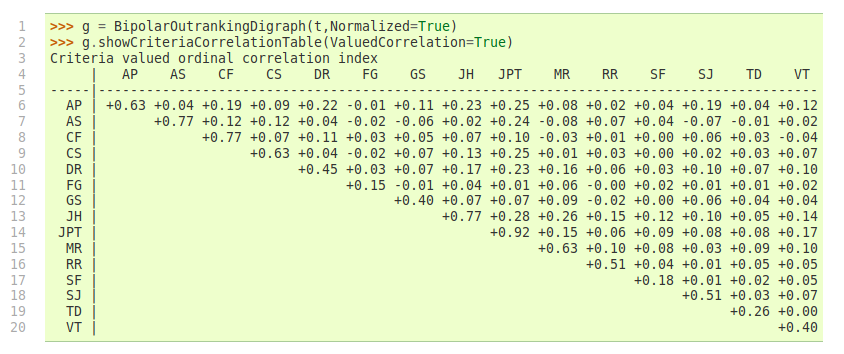
\includegraphics[width=12cm]{Figures/16-3-correlationTable.png}
\caption{Pairwise valued correlation of movie critics.} 
\label{fig:16.3}       % Give a unique label
\end{figure}

It is remarkable to notice in Fig.~\vref{fig:16.3} that, due to the quite numerous missing data, all pairwise valued ordinal correlation indexes $r(x\Leftrightarrow y)$ appear to be of low value, except the diagonal ones. These reflexive indexes $r(x\Leftrightarrow x)$ would trivially all amount to $+1.0$ in a plainly determined case. Here they indicate a reflexive normalized determination score $d$, i.e. the proportion of pairs of movies each critic did evaluate. Critic \texttt{JPT} (the editor of the Graffiti magazine), for instance, evaluated all but one ($d = 24\times23/600 = 0.92$), whereas critic \texttt{FG} evaluated only 10 movies among the 25 in discussion ($d = 10\times9/600 = 0.15$).

To get a picture of the actual divergence of rating opinions concerning jointly seen pairs of movies, we may develop a Principal Component Analysis of the corresponding $\tau$ correlation matrix\footnote{The 3D PCA plot method requires a running R statistics software  (https://www.r-project.org/) installation and the Calmat matrix calculator (see the \texttt{calmat} directory in the \Digraph resources)}. The 3D plot of the first 3 principal axes is shown in Fig.~\vref{fig:16.2}.\index{export3DplotOfCriteriaCorrelation@\texttt{export3DplotOfCriteriaCorrelation()}}
\begin{lstlisting}
>>> bod.export3DplotOfCriteriaCorrelation(\
...                     ValuedCorrelation=False)
\end{lstlisting}
\begin{figure}[h]
%\sidecaption
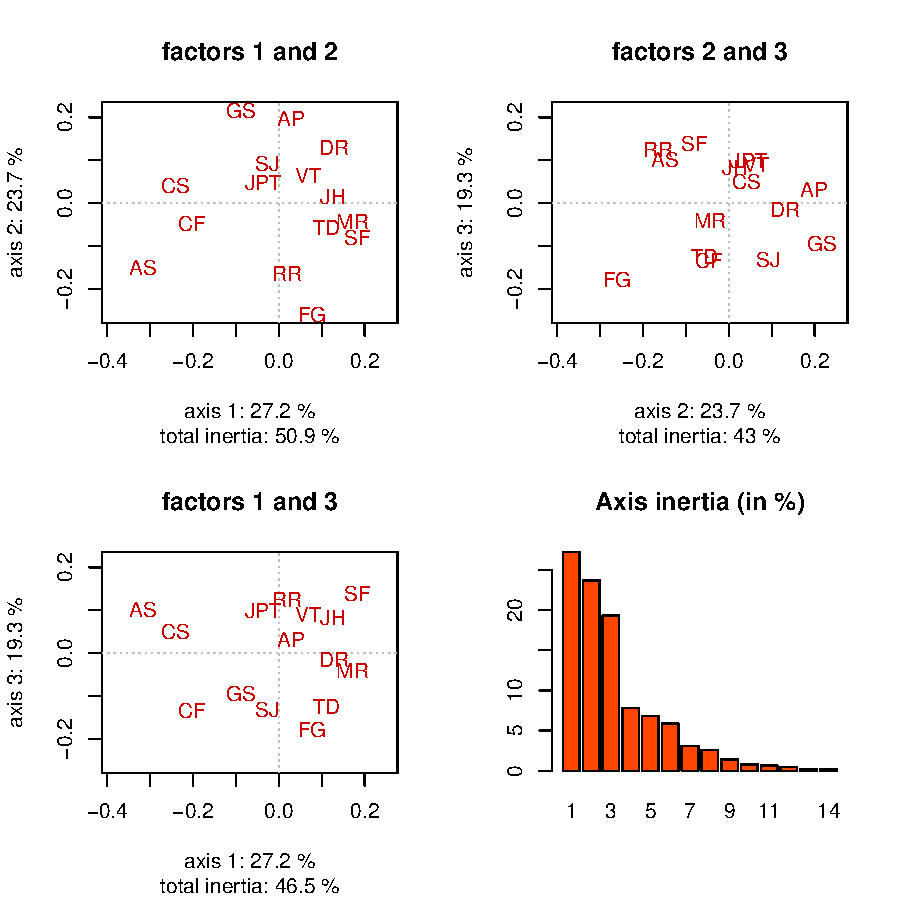
\includegraphics[width=10cm]{Figures/16-4-correlationPCA.pdf}
\caption{3D PCA plot of the criteria ordinal correlation matrix.}
\label{fig:16.4}       % Give a unique label
\end{figure}
The first 3 principal axes support together about $70\%$ of the total inertia. Most eccentric and opposed in their respective rating opinions appear, on the first principal axis with $27.2\%$ inertia, the conservative daily press against labour and public press. On the second principal axis with $23.7.7\%$ inertia, it is the people press versus the cultural critical press. And, on the third axis with still $19.3\%$ inertia, the written media appear most opposed to the radio media.

\section{Exploring the ``\emph{better rated}''  and the ``\emph{as well as rated}'' opinions}
\label{sec:16.5}

In order to furthermore study the quality of a ranking result, it may be interesting to have a separate view on the asymmetric and symmetric parts of the ``\emph{at least as well rated as}'' opinions (see Section \vref{sec:2.3}).

Let us first inspect the pairwise asymmetric part, namely the ``\emph{better rated than}'' and ``\emph{less well rated than}'' opinions of the movie critics. \index{AsymmetricPartialDigraph@\texttt{AsymmetricPartialDigraph} class}
\begin{lstlisting}
>>> from digraphs import AsymmetricPartialDigraph
>>> ag = AsymmetricPartialDigraph(bod)
>>> ag.showHTMLRelationTable(\
...    actionsList=g.computeNetFlowsRanking(),ndigits=0)
\end{lstlisting}
\begin{figure}[h]
%\sidecaption
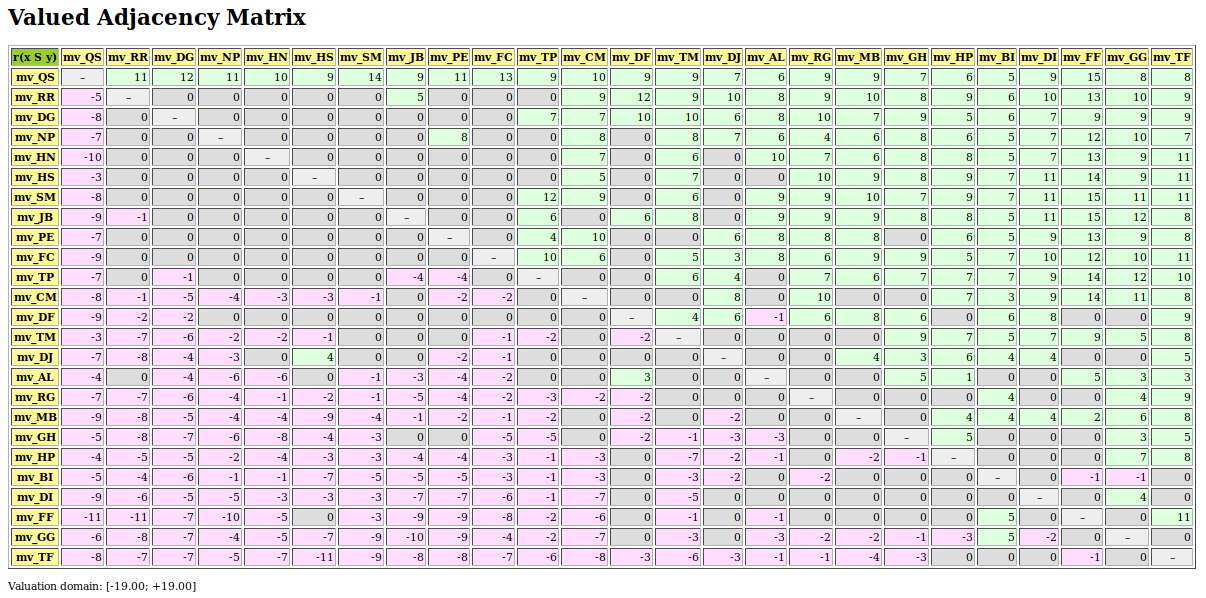
\includegraphics[width=12cm]{Figures/16-5-asymmetricPart.png}
\caption{Asymmetric part of \emph{graffiti07} digraph}
\label{fig:16.5}       % Give a unique label
\end{figure}

We notice in Fig.~\vref{fig:16.5} that the \NetFlows ranking rule inverts in fact just three ``\emph{less well rated than}'' opinions and four ``\emph{better rated than}'' ones. A similar look in Fig.~\vref{fig:16.6} at the symmetric part --the pairwise ``\emph{as well rated as}'' opinions-- suggests a preordered preference structure in several equivalently rated classes. \index{SymmetricPartialDigraph@\texttt{SymmetricPartialDigraph} class}
\begin{lstlisting}
>>> from digraphs import SymmetricPartialDigraph
>>> sg = SymmetricPartialDigraph(bod)
>>> sg.showHTMLRelationTable(\
...          actionsList=g.computeNetFlowsRanking(),\
...          ndigits=0)
\end{lstlisting}
\begin{figure}[h]
%\sidecaption
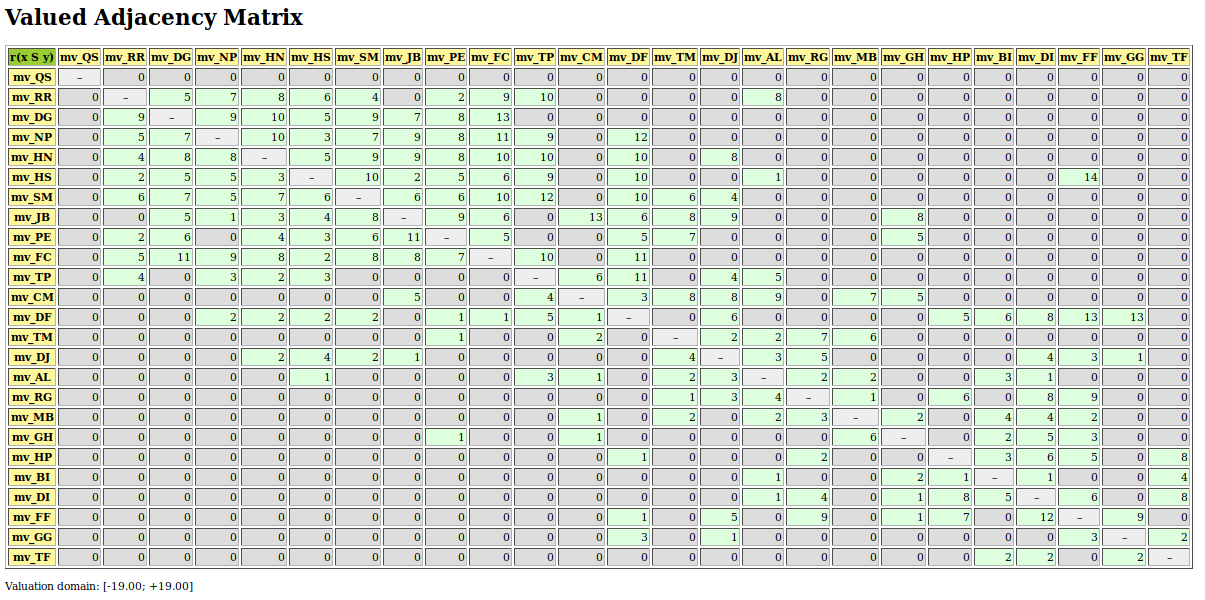
\includegraphics[width=12cm]{Figures/16-6-symmetricPart.png}
\caption{Symmetric part of \emph{graffiti07} digraph}
\label{fig:16.6}       % Give a unique label
\end{figure}

Such a preordering of the movies may, for instance, be computed with the \texttt{compute\-RankingByChoosing()} method\index{computeRankingByChoosing@\texttt{computeRankingByChoosing()}}, where we iteratively extract dominant kernels --best remaining choices-- and absorbent kernels --worst remaining choices-- (see the next Chapter). We operate therefore on the asymmetric ``\emph{better rated than}'' opinions, i.e. the codual of the ``\emph{at least as well rated as}'' opinions \footnote{A kernel in a digraph $g$ is a clique in the dual digraph $-g$.} (see Line 2 in List.~\vref{list:16.11}).
\begin{lstlisting}[caption={Bipolar ranking-by-choosing the Grafitti movies},label=list:16.11]
>>> from transitiveDigraphs import RankingByChoosingDigraph
>>> rbc = RankingByChoosingDigraph(bod,CoDual=True)
>>> rbc.showRankingByChoosing()
  Ranking by Choosing and Rejecting
    1st Best Choice ['mv_QS']
      2nd Best Choice ['mv_DG','mv_FC','mv_HN','mv_HS','mv_NP',
                       'mv_PE','mv_RR','mv_SM']
	3rd Best Choice ['mv_CM','mv_JB','mv_TM']
          4th Best Choice ['mv_AL','mv_TP']
          4th Worst Choice ['mv_AL','mv_TP']
        3rd Worst Choice ['mv_GH','mv_MB','mv_RG']
      2nd Worst Choice ['mv_DF','mv_DJ','mv_FF','mv_GG']
    1st Worst Choice ['mv_BI','mv_DI','mv_HP','mv_TF']
\end{lstlisting}

In the next Chapter~\vref{sec:17}, we thouroughly discuss the computation of such kernels in bipolar-valued digraphs.

%%%%%%% The chapter bibliography
%\normallatexbib
\clearpage
%\phantomsection
%\addcontentsline{toc}{section}{Chapter Bibliography}
\bibliographystyle{spbasic}
%\typeout{}
\bibliography{03-backMatters/reference}
%\chapter{On measuring the fitness of a multiple criteria ranking}
\label{sec:16}

\abstract*{ Starting from a motivating decision problem about how to list, from the best to the worst, a set movies that are star-rated by journalists and movie critics, the chapter shows that \Kendall 's ordinal correlation index tau may be extended to a relational bipolar-valued equivalence measure of  bipolar-valued digraphs. This finding gives way, on the one hand, to measure the fitness and fairness of multiple criteria ranking rules. On the other hand, it provides a tool for illustrating preference divergences between decision objectives and criteria.}

\abstract{ Starting from a motivating decision problem about how to list, from the best to the worst, a set movies that are star-rated by journalists and movie critics, the chapter shows that \Kendall 's ordinal correlation index tau may be extended to a relational bipolar-valued equivalence measure of  bipolar-valued digraphs. This finding gives way, on the one hand, to measure the fitness and fairness of multiple criteria ranking rules. On the other hand, it provides a tool for illustrating preference divergences between decision objectives and criteria.}

\section{Listing movies from best star-rated to worst}
\label{sec:16.1}

In a stubborn keeping with a two-valued logic, where every argument can only be true or false, there is no place for efficiently taking into account missing data or logical indeterminateness. These cases are seen as problematic and, at best are simply ignored. Worst, in modern data science, missing data get often replaced with \emph{fictive} values, potentially falsifying hence all subsequent computations.

In social choice problems, voting abstentions are, however, frequently observed and represent a social expression that may be significant for revealing non represented social preferences. And, in marketing studies, interviewees will not always respond to all the submitted questions. Again, such abstentions do sometimes contain nevertheless valid information concerning consumer preferences.

Such a case is given with  a list of star-rated movies that could be seen in town in September 2003 (source: \emph{Graffiti Star wars}, Edition Revue Luxembourg, September 2007, p. 30.). The underlying performance tableau data, stored in a file named \texttt{graffiti07.py}\footnote{to be found in the \texttt{examples} directory of the \Digraph resources}, is shown below with the \texttt{showHTMLPerformance\-Tableau()} method\index{showHTMLPerformanceTableau@\texttt{showHTMLPerformanceTableau()}}  : 
\begin{lstlisting}
>>> from outrankingDigraphs import\
...                        PerformanceTableau 
>>> gt07 = PerformanceTableau('graffiti07')
>>> gt07.showHTMLPerformanceTableau(\
...               title='Graffiti Star wars',\
...               ndigits=0)
\end{lstlisting}
\begin{figure}[h]
%\sidecaption
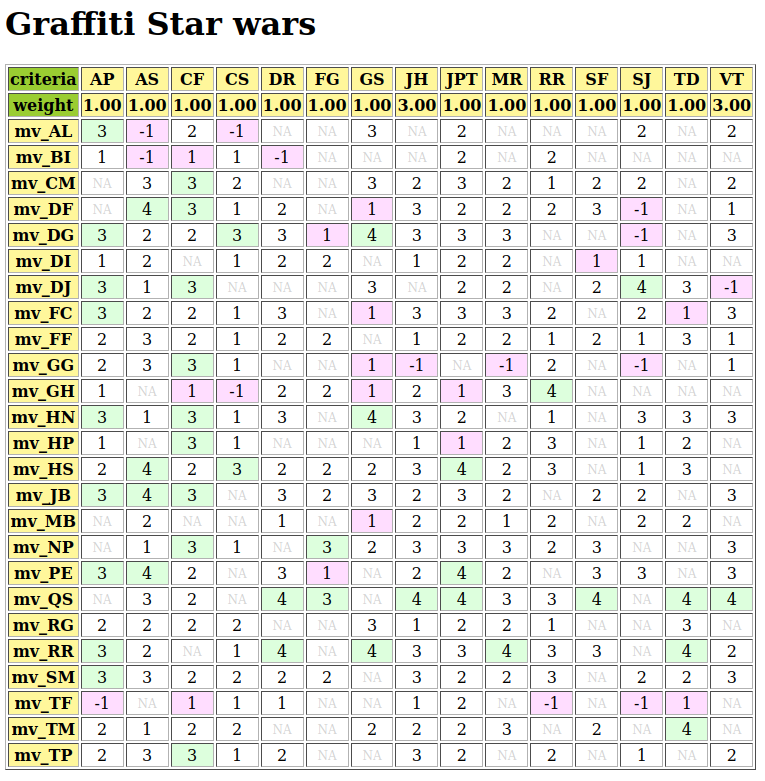
\includegraphics[width=11cm]{Figures/16-1-graffiti07_1.png}
\caption{\emph{Graffiti} magazine's movie ratings from September 2007}
\label{fig:16.1}       % Give a unique label
\end{figure}

Figure~\vref{fig:16.1} shows the star-ratings of $25$ movies by $15$ journalists and movie critics: $5$ stars (\emph{masterpiece}), $4$ stars (\emph{must be seen}), $3$ stars (\emph{excellent}), $2$ stars (\emph{good}), $1$ star (\emph{could be seen}), $-1$ star (\emph{I do not like}), $-2$ stars (\emph{I hate}), \texttt{NA} (\emph{not seen}). Notice in the second row the higher significance ($3.00$) that is granted to two locally renowned movie critics, namely \texttt{JH} and \texttt{VT}. Their opinion counts for three times the opinion of the other critics. With six times a 4 stars (\emph{must be seen}) grade, \texttt{mv\_QS} is best-rated, followed by \texttt{mv\_RR} with four times a 4 stars mark. Fewest stars obtains movie \texttt{mv\_TF} with three times a $-1$ star (\emph{don't like}) mark and five times a $1$ star mark. Notice that many movies, like movie \texttt{mv\_BI}, are only rated by some of the critics. 

To aggregate all the critics' star-ratings, the \emph{Graffiti} magazine computes for each movie a global score --the average weighted number of stars it obtained-- just ignoring the \emph{not seen} movies. Listing~\vref{list:16.1} illustrates below how to compute these global scores using the data stored in the \texttt{gt07} performance tableau. Attribute \texttt{gt07.actions}, resp. \texttt{gt07.criteria}, contains the description of the 25 movies, resp. the 15 critics. The actual star-ratings are to be found in the \texttt{gt07.evaluation} attribute.
\begin{lstlisting}[caption={Computing the average weighted number of stars per movie},label=list:16.1,basicstyle=\ttfamily\scriptsize]
>>> # gt07 = PerformanceTableau('graffiti07')
>>> globalScores = {}
>>> for mv in gt07.actions:
>>>     globalScores[mv] = Decimal('0')
>>>     sumWeights = Decimal('0')
>>>     for critic in gt07.criteria:
>>>         stars = gt07.evaluation[critic][mv]
>>>         if stars != gt07.NA:
>>>             weight = gt07.criteria[critic]['weight']
>>>             globalScores[mv] += (stars * weight)
>>>             sumWeights += weight
>>>     globalScores[mv] /= sumWeights
>>> graffitiList = [(globalScores[mv],mv) for mv in globalScores]
>>> graffitiList.sort(reverse=True)
>>> for item in graffitiList:
>>>     print('%s: %.2f' % (item[1],item[0]) )
  mv_QS: 3.60
  mv_RR: 2.88
  mv_PE: 2.67
  mv_JB: 2.62
  mv_HN: 2.62
  mv_NP: 2.60
  mv_HS: 2.60
  mv_DG: 2.56
  mv_SM: 2.53
  mv_FC: 2.41
  mv_TP: 2.21
  mv_CM: 2.20
  mv_TM: 2.17
  mv_DF: 1.94
  mv_RG: 1.83
  mv_MB: 1.73
  mv_GH: 1.67
  mv_DJ: 1.67
  mv_FF: 1.61
  mv_AL: 1.60
  mv_HP: 1.55
  mv_DI: 1.42
  mv_GG: 0.71
  mv_BI: 0.71
  mv_TF: 0.55
\end{lstlisting}

The global scrores ranking confirms in Lines 17-18 both leading movies --\texttt{mv\_QS} ($3.60$) and \texttt{mv\_RR} ($2.88$) -- as well as in Line 41 the weakest rated one --\texttt{mv\_TF} ($0.55$). Mind however that these global averages, due to the numerous missing grades, are not computed with commensurable denominators; some critics do indeed use a more or less extended range of stars. The movies not seen for instance by critic \texttt{SJ} are favoured, as this critic is severer than others in her rating. Dropping the movies that were not graded by all the critics is not possible either, as none of the $25$ movies was actually rated by all the $15$ critics. Providing a fictive value for the many not seen situations, will as well always somehow falsify the global scores. What to do?

A better approach is to rank the movies on the basis of pairwise bipolar-valued  ``\emph{rated at least as well as}'' statements. Under this epistemic argumentation approach, missing grades are naturally treated as opinion abstentions and hence do not falsify the logical computations. Such a \NetFlows ranking from best-rated to weakest-rated is provided by the \textbf{heatmap} browser view generated with the \texttt{showHTMLPerformanceHeatmap()} method\index{showHTMLPerformanceHeatmap@\texttt{showHTMLPerformanceHeatmap()}} (see List.~\vref{list:16.2}).
\begin{lstlisting}[caption={Showing the movie from best to worst rated in a heatmap view},label=list:16.2]
>>> gt07.showHTMLPerformanceHeatmap(\
...            pageTitle='Ranking the movies',\  
...            rankingRule='NetFlows',
...            Correlations=True,\
...            ndigits=0)
\end{lstlisting}
\begin{figure}[h]
%\sidecaption
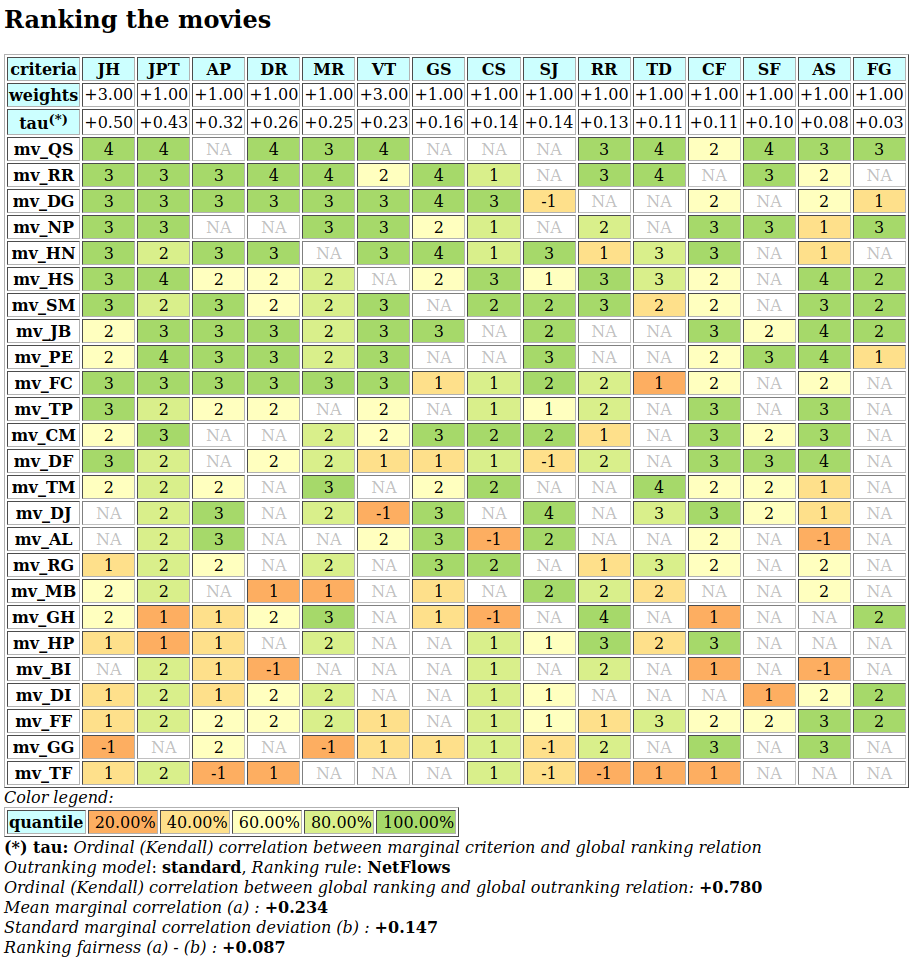
\includegraphics[width=11cm]{Figures/16-2-graffiti07_2.png}
\caption{\emph{Graffiti} magazine's movie ratings from September 2007 ranked with the \NetFlows rule}
\label{fig:16.2}       % Give a unique label
\end{figure}

The \NetFlows ranking shown in Fig.~\vref{fig:16.2} confirms again that movie \texttt{mv\_QS}, with $6$ \emph{must be seen} marks, is correctly best-ranked and the movie \texttt{mv\_TF} is worst-ranked with five \emph{don't like} marks. 

It is fair, however, to eventually mention here that the \emph{Graffiti} magazine's average stars ranking rule is actually showing a very similar result. Indeed, average scores usually confirm well all evident pairwise comparisons, yet \emph{enforce} comparability for all less evident ones. How to judge now the fitness of a given ranking rule?

This is the purpose of the ordinal correlation \emph{tau} indexes shown in Fig.~\vref{fig:16.2} 3rd row. Computing these ordinal correlation indexes is the subject of the next Section.
 
\section{\Kendall 's ordinal correlation tau index}
\label{sec:16:2}

M. G. Kendall\index{Kendall@\emph{Kendall M.G.}} defined his ordinal correlation $\tau$ (\emph{tau}) index for linear orders of dimension $n$ as a balancing of the number $Co$ of correctly oriented pairs against the number $In$ of incorrectly oriented pairs \citep{KEN-1938}. The total number of irreflexive pairs being $n(n-1)$, in the case of linear orders, $Co + In \;=\; n(n-1)$.  Hence $\tau \;=\; \big(\frac{Co}{n(n-1)}\big) \,-\, \big(\frac{In}{n(n-1)}\big)$. In case $In$ is zero, $\tau \;=\; +1$  (all pairs are equivalently oriented); inversely, in case $Co$ is zero, $\tau \;=\; -1$ (all pairs are differently oriented).

Noticing that $\frac{Co}{n(n-1)} \;=\; 1 \,-\, \frac{In}{n(n-1)}$, and recalling that the bipolar-valued negation is operated by changing the sign of the characteristic value:
\begin{equation}
      \tau \;=\; 1 -2\frac{In}{n(n-1)} \;=\; -\big(\,2\frac{In}{n(n-1)} \,-\, 1\,\big) \;=\; 2\frac{Co}{n(n-1)} \,-\, 1,
\end{equation} 
\Kendall 's original \emph{tau} definition implemented in fact the bipolar-valued negation of the non equivalence of two linear orders, i.e. the normalized majority margin of equivalently oriented irreflexive pairs.

Let \texttt{r1} and \texttt{r2} be two random crisp relations defined on a same set of 5 alternatives. We may compute \Kendall 's \emph{tau} index as shown in List.~\vref{list:16.3}.
\begin{lstlisting}[caption={Computing a relational equivalence digraph},label=list:16.3]
>>> from randomDigraphs import RandomDigraph
>>> r1 = RandomDigraph(order=5,Bipolar=True)
>>> r2 = RandomDigraph(order=5,Bipolar=True)
>>> from digraphs import EquivalenceDigraph
>>> eqd = EquivalenceDigraph(r1,r2)
>>> eqd.showRelationTable(ReflexiveTerms=False)
  * ---- Relation Table -----
  r(<=>)|  'a1'	  'a2'	  'a3'	  'a4'	  'a5'	  
  ------|-------------------------------------
   'a1' |    -   -1.00   1.00   -1.00    1.00	 
   'a2' |  -1.00   -    -1.00    1.00   -1.00	 
   'a3' |  -1.00 -1.00    -      1.00    1.00	 
   'a4' |  -1.00  1.00  -1.00     -      1.00	 
   'a5' |  -1.00  1.00  -1.00    1.00     - 	 
   Valuation domain: [-1.00;1.00]
>>> eqd.correlation
  {'correlation': -0.1, 'determination': 1.0}
\end{lstlisting}
In the table of the equivalence relation $(\mathtt{r1}\, \Leftrightarrow\, \mathtt{r2})$ above (see List.~\vref{list:16.1} Lines 10-14), we observe that the normalized majority margin of equivalent versus non equivalent irreflexive pairs amounts to $(9 - 11)/20 = -0.1$, i.e. the value of \Kendall 's \emph{tau} index in this plainly determined crisp case (see Line 17).

What happens now with more or less determined and even partially indeterminate relations? May we proceed in a similar way?

\section{Bipolar-valued relational equivalence}
\label{sec:16.3}

Two random bipolar-valued digraphs \texttt{d1} and \texttt{d2} of order five, generated in List.~\vref{list:16.4}, will help exploring this idea.
\begin{lstlisting}[caption={Two random bipolar-valued digraphs},label=list:16.4]
>>> from randomDigraphs import RandomValuationDigraph
>>> d1 = RandomValuationDigraph(order=5,seed=1)
>>> d1.showRelationTable(ReflexiveTerms=False)
  * ---- Relation Table -----
   r(d1)|   'a1'   'a2'   'a3'   'a4'   'a5'	  
  ------|------------------------------------
   'a1' |    - 	  -0.66	  0.44	  0.94	-0.84	 
   'a2' |  -0.36    - 	 -0.70	  0.26	 0.94	 
   'a3' |   0.14   0.20	   - 	  0.66	-0.04	 
   'a4' |  -0.48 - 0.76	  0.24	   -  	-0.94	 
   'a5' |  -0.02   0.10	  0.54	  0.94    - 	 
   Valuation domain: [-1.00;1.00]
>>> d2 = RandomValuationDigraph(order=5,seed=2)
>>> d2.showRelationTable(ReflexiveTerms=False)
  * ---- Relation Table -----
   r(d2)|   'a1'   'a2'   'a3'   'a4'   'a5'	  
  ------|-----------------------------------
   'a1' |   -     -0.86  -0.78  -0.80  -0.08	 
   'a2' |  -0.58    -     0.88   0.70  -0.22	 
   'a3' |  -0.36   0.54    -    -0.46   0.54	 
   'a4' |  -0.92   0.48   0.74    -    -0.60	 
   'a5' |   0.10   0.62   0.00   0.84    - 	 
   Valuation domain: [-1.00;1.00]
\end{lstlisting}
In the generated random digraphs \texttt{d1} and \texttt{d2}, 9 pairs, like \texttt{(a1,a2)} or \texttt{(a3,a2)} for instance, appear equivalently oriented (see Lines 7,18 or 9,20). The \texttt{Equiva\-lenceDigraph} class\index{EquivalenceDigraph@\texttt{EquivalenceDigraph} class} computes this bipolar-valued relational equivalence between digraphs \texttt{d1} and \texttt{d2} (see List.~\vref{list:16.5}).
\begin{lstlisting}[caption={Bipolar-valued Equivalence Digraph},label=list:16.5]
>>> from digraphs import EquivalenceDigraph
>>> eqd = EquivalenceDigraph(d1,d2)
>>> eqd.showRelationTable(ReflexiveTerms=False)
  * ---- Relation Table -----
   r(<=>)|  'a1'  'a2'   'a3'   'a4'   'a5'	  
   ------|---------------------------------
   'a1' |   - 	  0.66  -0.44  -0.80   0.08	 
    'a2' |  0.36   -    -0.70   0.26  -0.22	 
    'a3' | -0.14  0.20    -    -0.46  -0.04	 
    'a4' |  0.48 -0.48   0.24    -     0.60	 
    'a5' | -0.02  0.10   0.00   0.84    - 	 
   Valuation domain: [-1.00;1.00]
\end{lstlisting}

In our bipolar-valued epistemic logic, logical disjunctions and conjunctions are implemented as $\max$, respectively $\min$ operations. Notice also that the logical equivalence $(\mathtt{d1}\, \Leftrightarrow\, \mathtt{d2})$ corresponds to a double implication $(\mathtt{d1}\, \Rightarrow\, \mathtt{d2})\; \wedge \; (\mathtt{d2}\, \Rightarrow\,  \mathtt{d1})$ and that the implication $(\mathtt{d1} \Rightarrow \mathtt{d2})$ is logically equivalent to the disjunction $(\neg \mathtt{d1} \vee \mathtt{d2})$.

When $r(x\,\mathtt{d1}\, y)$ and $r(x\,\mathtt{d2}\; y)$ denote the bipolar-valued characteristic values of relation \texttt{d1}, resp. \texttt{d2}, we may hence compute as follows a majority margin $M(\mathtt{d1} \Leftrightarrow \mathtt{d2})$ between equivalently and not equivalently oriented irreflexive pairs $(x,y)$:
\begin{equation}\label{eq:16:2}
  \begin{split}
&M(\mathtt{d1} \Leftrightarrow \mathtt{d2}) \; =\\
&\quad \quad \sum_{(x \neq y)} \Big[ \min \Big( \max \big( -r(x \,\mathtt{d1}\, y), r(x \,\mathtt{d2}\, y)\big), \max \big( -r(x \,\mathtt{d2}\, y), r(x \,\mathtt{d1}\, y)\big) \Big) \Big]\;.
\end{split}
\end{equation}

$M(\mathtt{d1} \Leftrightarrow \mathtt{d2})$ is thus given by the sum of the non reflexive terms of the relation table of $eqd$, the relational equivalence digraph computed above (see List.~\vref{list:16.5}). In the crisp case, $M(\mathtt{d1}\,\Leftrightarrow\, \mathtt{d2})$  is normalized with the maximum number of possible irreflexive pairs, namely $n(n-1)$. In the extended $r$-valued case, the maximal possible equivalence majority margin $M$ corresponds to the sum $D$ of the conjoint determinations of $(x \,\mathtt{d1}\, y)$ and $(x \,d2\, y)$ (see \citet{BIS-2012a}):
\begin{equation}
  D \;=\; \sum_{x \neq y} \min \Big[ abs\big(r(x \,\mathtt{d1}\, y) \big), abs \big( r(x \,\mathtt{d2}\, y \big)  \Big]\;,
\end{equation}
and we obtain hence in the general $r$ -valued case:
\begin{equation}\label{eq:16.4}
  \tau(\mathtt{d1},\mathtt{d2}) \;=\; \frac{M(\mathtt{d1}\,\Leftrightarrow\, \mathtt{d2})}{D}\;.
\end{equation}

$\tau(\mathtt{d1},\mathtt{d2})$ corresponds so to the classical ordinal correlation index, yet restricted to the conjointly determined parts of the given digraphs $\mathtt{d1}$ and $\mathtt{d2}$. In the limit case of two crisp linear orders, $D$ equals $n(n-1)$, i.e. the number of irreflexive pairs, and we recover \Kendall 's original \emph{tau} index definition.

It is worthwhile noticing that the ordinal correlation index $\tau(\mathtt{d1},\mathtt{d2})$ one obtains above corresponds in fact to the ratio of:
\begin{itemize}
\item $r(\mathtt{d1}\,\Leftrightarrow\, \mathtt{d2}) \;=\; \frac{M(\mathtt{d1}\,\Leftrightarrow\, \mathtt{d2})}{n(n-1)}$:\\the normalized majority margin of the pairwise \emph{relational} equivalence statements, also called \emph{valued ordinal correlation}, and 
\item $d \;=\; \frac{D}{n(n-1)}$:\\ the normalized determination of the corresponding pairwise relational equivalence statements, in fact the \emph{determinateness} of the relational equivalence digraph.
\end{itemize}

The epistemic determination effect is thus successfully \emph{out-factored} from the ordinal correlation effect. With completely determined relations, $\tau(\mathtt{d1},\mathtt{d2}) \;=\; r(\mathtt{d1}\,\Leftrightarrow\, \mathtt{d2})$. The ordinal correlation with a completely indeterminate digraph, i.e. when $D = 0$, is set by convention to the indeterminate correlation value $0.0$. With uniformly chosen random $r$-valued digraphs, the expected $\tau$ index is $0.0$, denoting in fact an indeterminate relational equivalence. The corresponding expected normalized determination $d$ is about $0.333$ (see \citep{BIS-2012a}).

We may below verify Eq.~\vref{eq:6.4} with help of the equivalence digraph $eqd$ computed in List.~\vref{list:16.5}.
\begin{lstlisting}[caption={Computing the ordinal correlation index from the equivalence digraph},label=list:16.6]
>>> # eqd = EquivalenceDigraph(d1,d2)
>>> M = Decimal('0'); D = Decimal('0')
>>> n2 = eqd.order*(eqd.order - 1)
>>> for x in eqd.actions:
...     for y in eqd.actions:
...         M += eqd.relation[x][y]
...         D += abs(eqd.relation[x][y])
>>> print('r(rd1<=>rd2) = %+.3f, d = %.3f, tau = %+.3f' %\
          (M/n2,D/n2,M/D))   
  r(rd1<=>rd2) = +0.026, d = 0.356, tau = +0.073  
\end{lstlisting}

The \Digraph resources directly provide for the preceding computations the \texttt{compute\-OrdinalCorrelation()} method\index{computeOrdinalCorrelation@\texttt{computeOrdinalCorrelation()}} which renders a dictionary with a \texttt{correlation} ($\tau$) and a \texttt{determina\-tion} ($d$) attribute. We may recover $r(d1\,\Leftrightarrow\, d2)$ by multiplying $\tau$ with $d$ (see List.~\vref{list:16.7} Line 4). 
\begin{lstlisting}[caption={Computing the valued ordinal correlation index},label=list:16.7]
>>> corrd1d2 = d1.computeOrdinalCorrelation(d2)
>>> tau = corrd1d2['correlation']
>>> d = corrd1d2['determination']
>>> r = tau * d
>>> print('tau(d1,d2) = %+.3f, d = %.3f,\
...        r(d1<=>d2) = %+.3f' % (tau, d, r))
  tau(d1,d2) = +0.073, d = 0.356, r(d1<=>d2) = +0.026
\end{lstlisting}

The \Digraph resources provide for convenience a direct \texttt{showCorrela\-tion()} method\index{showCorrelation@\texttt{showCorrelation()}}:
\begin{lstlisting}
>>> d1.showCorrelation(\
...       d1.computeOrdinalCorrelation(d2) )
  Correlation indexes:
    Extended Kendall tau       : +0.073
    Epistemic determination    :  0.356
    Bipolar-valued equivalence : +0.026
\end{lstlisting}

We are now ready for assessing the quality of the \NetFlows ranking of the movies shown in the heat map view of Fig.~\vref{fig:16.2}. 

\section{Fitness of ranking heuristics}
\label{sec:16.3}

The \NetFlows ranking of the movies shown in the heatmap view in Fig.~\vref{fig:16.2} is based on the bipolar-valued outranking digraph modelling the pairwise global ``\emph{rated at least as well as}'' relation among the $25$ movies from the performance tableau instance \texttt{gt07}.
\begin{lstlisting}[caption={The bipolar-valued outranking digraph of the star-rated movies},label=list:16.8]
>>> bod = BipolarOutrankingDigraph(gt07)
  *------- Object instance description ------*
   Instance class   : BipolarOutrankingDigraph
   Instance name    : rel_grafittiPerfTab.xml
   Actions          : 25
   Criteria         : 15
   Size             : 390
   Determinateness  : 65%
   Valuation domain : {'min': Decimal('-1.0'),
                       'med': Decimal('0.0'),
                       'max': Decimal('1.0'),}
>>> g.computeCoSize()
  188
\end{lstlisting}
Listing~\vref{list:16.8} reveals that the outranking digraph \texttt{bod} contains $390$ positively validated (Line 7), $188$ positively invalidated (Line 13)\index{computeCoSize@\texttt{computeCoSize()}}, and 22 indeterminate outranking situations from the potential $25 \times 24 = 600$ irreflexive movie pairs.

Listing~\vref{list:16.9} illustrates with the \texttt{NetFlowsOrder} class \index{NetFlowsOrder@\texttt{NetFlowsOrder} class} from the \texttt{linearOr\-ders} module\index{linearOrders@\texttt{linearOrders} module} how to compute the global \NetFlows ranking \texttt{nf}, as shown in the ordered heat map of Fig.~\vref{fig:16.2} and the bipolar-valued relational equivalence of the \texttt{nf} ranking with each one the individual critic's star-ratings.
\begin{lstlisting}[caption={Computing marginal criterion correlations with global \NetFlows ranking},label=list:16.9]
>>> from linearOrders import NetFlowsOrder
>>> nf = NetFlowsOrder(bod)
>>> nf.netFlowsRanking
  ['mv_QS', 'mv_RR', 'mv_DG', 'mv_NP', 'mv_HN', 'mv_HS', 'mv_SM',
   'mv_JB', 'mv_PE', 'mv_FC', 'mv_TP', 'mv_CM', 'mv_DF', 'mv_TM',
   'mv_DJ', 'mv_AL', 'mv_RG', 'mv_MB', 'mv_GH', 'mv_HP', 'mv_BI',
   'mv_DI', 'mv_FF', 'mv_GG', 'mv_TF']
>>> for i,item in enumerate(\
...       bod.computeMarginalVersusGlobalRankingCorrelations(\
...              nf.netFlowsRanking,ValuedCorrelation=True) ):\
...     print('r(%s<=>nf) = %+.3f' % (item[1],item[0]) )   

  r(JH<=>nf)  = +0.500
  r(JPT<=>nf) = +0.430
  r(AP<=>nf)  = +0.323
  r(DR<=>nf)  = +0.263
  r(MR<=>nf)  = +0.247
  r(VT<=>nf)  = +0.227
  r(GS<=>nf)  = +0.160
  r(CS<=>nf)  = +0.140
  r(SJ<=>nf)  = +0.137
  r(RR<=>nf)  = +0.133
  r(TD<=>nf)  = +0.110
  r(CF<=>nf)  = +0.110
  r(SF<=>nf)  = +0.103
  r(AS<=>nf)  = +0.080
  r(FG<=>nf)  = +0.027
\end{lstlisting}

In List.~\vref{list:16.9} (see Lines 13-27), we obtain the relational equivalence characteristic values shown in the third row of the ranked heatmap (see Fig.~\vref{fig:16.2}). The global \NetFlows ranking \texttt{nf} represents obviously a rather balanced compromise with respect to each movie critic's star-ratings, as there appears no negative correlation with anyone of them. The ranking \texttt{nf} apparently takes also correctly in account that the journalist $JH$, a locally renowned movie critic, shows a higher significance weight (see Line 13).

The ordinal correlation between the global \NetFlows ranking and the outranking digraph \texttt{bod} may be furthermore computed as illstrated in List.~\vref{list:16.10}: 
\begin{lstlisting}[caption={Computing the ordinal correlation between \NetFlows and global outranking digraph},label=list:16.10]
>>> corrgnf = bod.computeOrdinalCorrelation(nf)
>>> bod.showCorrelation(corrgnf)
  Correlation indexes:
    Extended Kendall tau       : +0.780
    Epistemic determination    :  0.300
    Bipolar-valued equivalence : +0.234
\end{lstlisting}
One may notice in Line 4 that the ordinal correlation $\tau(\mathtt{bod},\mathtt{nf})$ index between the \NetFlows ranking $\mathtt{nf}$ and the determined part of the outranking digraph $\mathtt{bod}$ is quite high ($+0.78$). Due to the rather high number of missing data, the $r$ -valued relational equivalence between the $\mathtt{nf}$ and the $\mathtt{bod}$ digraph, with a characteristics value of only $+0.234$, may be misleading. Yet, $+0.234$ still corresponds to a $62\%$ majority support of the movie critics' star-ratings.

It would be interesting to compare similarly the correlations one may obtain with other global ranking heuristics, like the \Copeland ranking rule.

\section{Illustrating preference divergences}
\label{sec:16.4}

The bipolar-valued relational equivalence indexes gives us, via the \texttt{showCrite\-riaCorrelationTable(ValuedCorrelation=True)} method\index{showCriteriaCorrelationTable@\texttt{showCriteriaCorrelationTable()}}, a further measure for studying how \emph{divergent} may appear the rating opinions expressed by the movie critics. 
\begin{figure}[h]
%\sidecaption
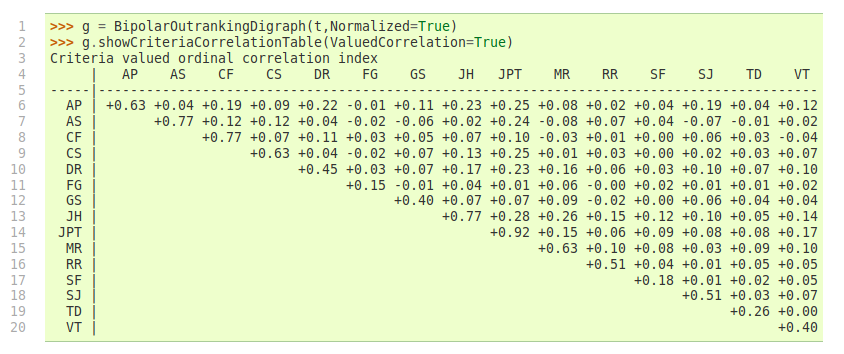
\includegraphics[width=12cm]{Figures/16-3-correlationTable.png}
\caption{Pairwise valued correlation of movie critics.} 
\label{fig:16.3}       % Give a unique label
\end{figure}

It is remarkable to notice in Fig.~\vref{fig:16.3} that, due to the quite numerous missing data, all pairwise valued ordinal correlation indexes $r(x\Leftrightarrow y)$ appear to be of low value, except the diagonal ones. These reflexive indexes $r(x\Leftrightarrow x)$ would trivially all amount to $+1.0$ in a plainly determined case. Here they indicate a reflexive normalized determination score $d$, i.e. the proportion of pairs of movies each critic did evaluate. Critic \texttt{JPT} (the editor of the Graffiti magazine), for instance, evaluated all but one ($d = 24\times23/600 = 0.92$), whereas critic \texttt{FG} evaluated only 10 movies among the 25 in discussion ($d = 10\times9/600 = 0.15$).

To get a picture of the actual divergence of rating opinions concerning jointly seen pairs of movies, we may develop a Principal Component Analysis of the corresponding $\tau$ correlation matrix\footnote{The 3D PCA plot method requires a running R statistics software  (https://www.r-project.org/) installation and the Calmat matrix calculator (see the \texttt{calmat} directory in the \Digraph resources)}. The 3D plot of the first 3 principal axes is shown in Fig.~\vref{fig:16.2}.\index{export3DplotOfCriteriaCorrelation@\texttt{export3DplotOfCriteriaCorrelation()}}
\begin{lstlisting}
>>> bod.export3DplotOfCriteriaCorrelation(\
...                     ValuedCorrelation=False)
\end{lstlisting}
\begin{figure}[h]
%\sidecaption
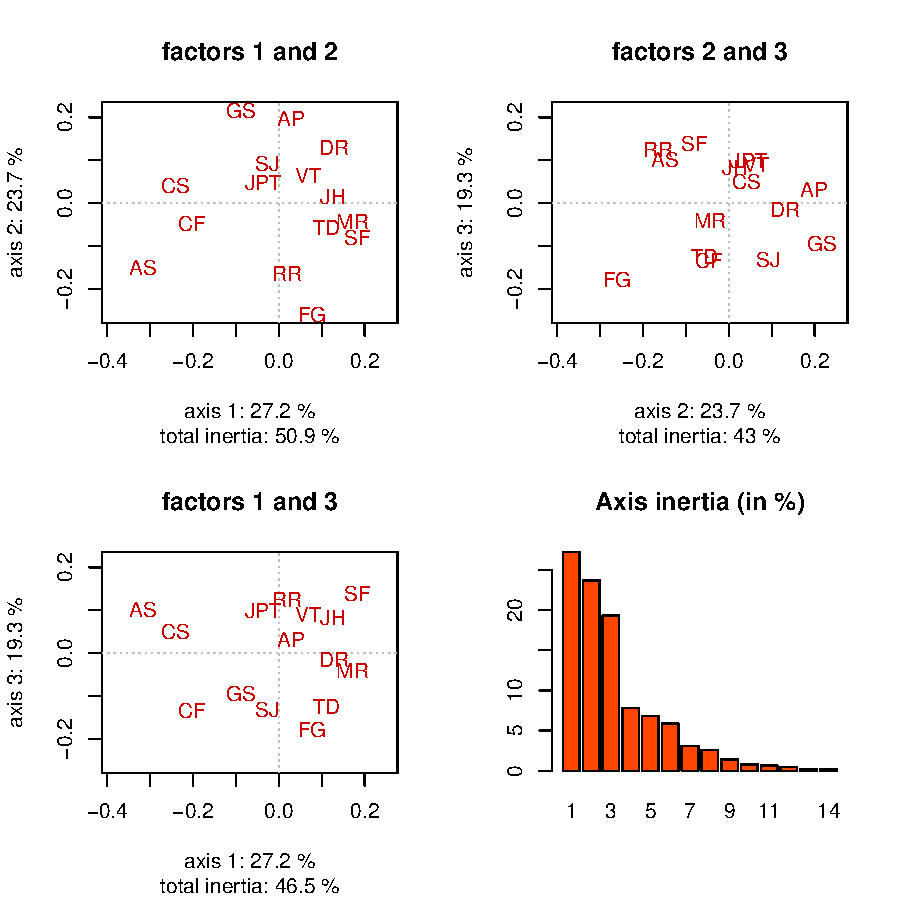
\includegraphics[width=10cm]{Figures/16-4-correlationPCA.pdf}
\caption{3D PCA plot of the criteria ordinal correlation matrix.}
\label{fig:16.4}       % Give a unique label
\end{figure}
The first 3 principal axes support together about $70\%$ of the total inertia. Most eccentric and opposed in their respective rating opinions appear, on the first principal axis with $27.2\%$ inertia, the conservative daily press against labour and public press. On the second principal axis with $23.7.7\%$ inertia, it is the people press versus the cultural critical press. And, on the third axis with still $19.3\%$ inertia, the written media appear most opposed to the radio media.

\section{Exploring the ``\emph{better rated}''  and the ``\emph{as well as rated}'' opinions}
\label{sec:16.5}

In order to furthermore study the quality of a ranking result, it may be interesting to have a separate view on the asymmetric and symmetric parts of the ``\emph{at least as well rated as}'' opinions (see Section \vref{sec:2.3}).

Let us first inspect the pairwise asymmetric part, namely the ``\emph{better rated than}'' and ``\emph{less well rated than}'' opinions of the movie critics. \index{AsymmetricPartialDigraph@\texttt{AsymmetricPartialDigraph} class}
\begin{lstlisting}
>>> from digraphs import AsymmetricPartialDigraph
>>> ag = AsymmetricPartialDigraph(bod)
>>> ag.showHTMLRelationTable(\
...    actionsList=g.computeNetFlowsRanking(),ndigits=0)
\end{lstlisting}
\begin{figure}[h]
%\sidecaption
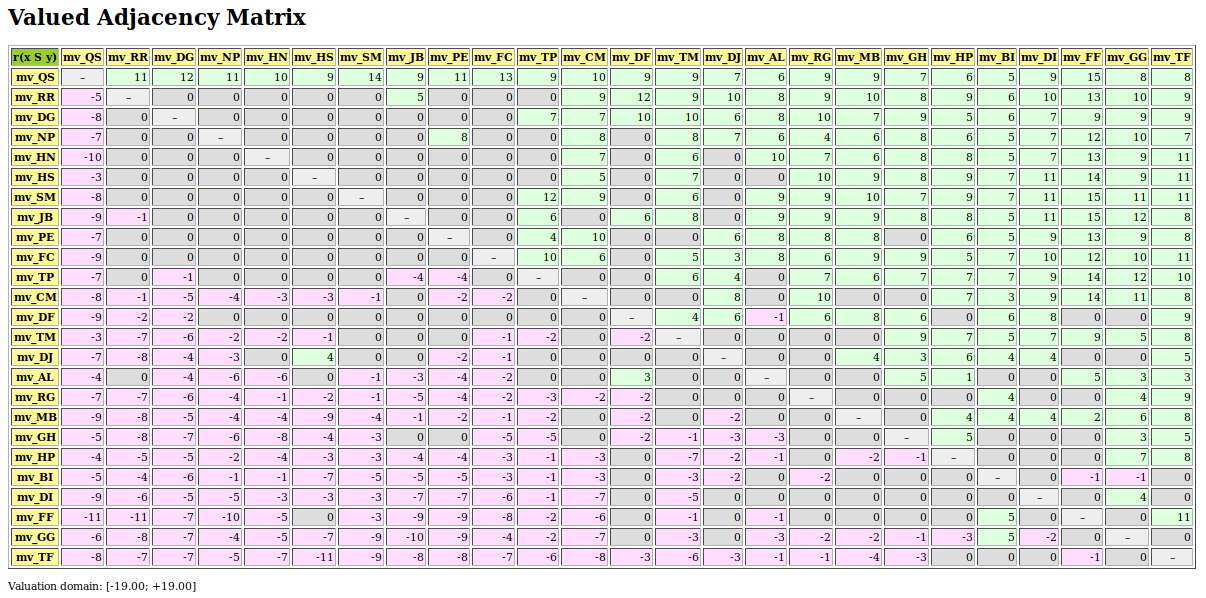
\includegraphics[width=12cm]{Figures/16-5-asymmetricPart.png}
\caption{Asymmetric part of \emph{graffiti07} digraph}
\label{fig:16.5}       % Give a unique label
\end{figure}

We notice in Fig.~\vref{fig:16.5} that the \NetFlows ranking rule inverts in fact just three ``\emph{less well rated than}'' opinions and four ``\emph{better rated than}'' ones. A similar look in Fig.~\vref{fig:16.6} at the symmetric part --the pairwise ``\emph{as well rated as}'' opinions-- suggests a preordered preference structure in several equivalently rated classes. \index{SymmetricPartialDigraph@\texttt{SymmetricPartialDigraph} class}
\begin{lstlisting}
>>> from digraphs import SymmetricPartialDigraph
>>> sg = SymmetricPartialDigraph(bod)
>>> sg.showHTMLRelationTable(\
...          actionsList=g.computeNetFlowsRanking(),\
...          ndigits=0)
\end{lstlisting}
\begin{figure}[h]
%\sidecaption
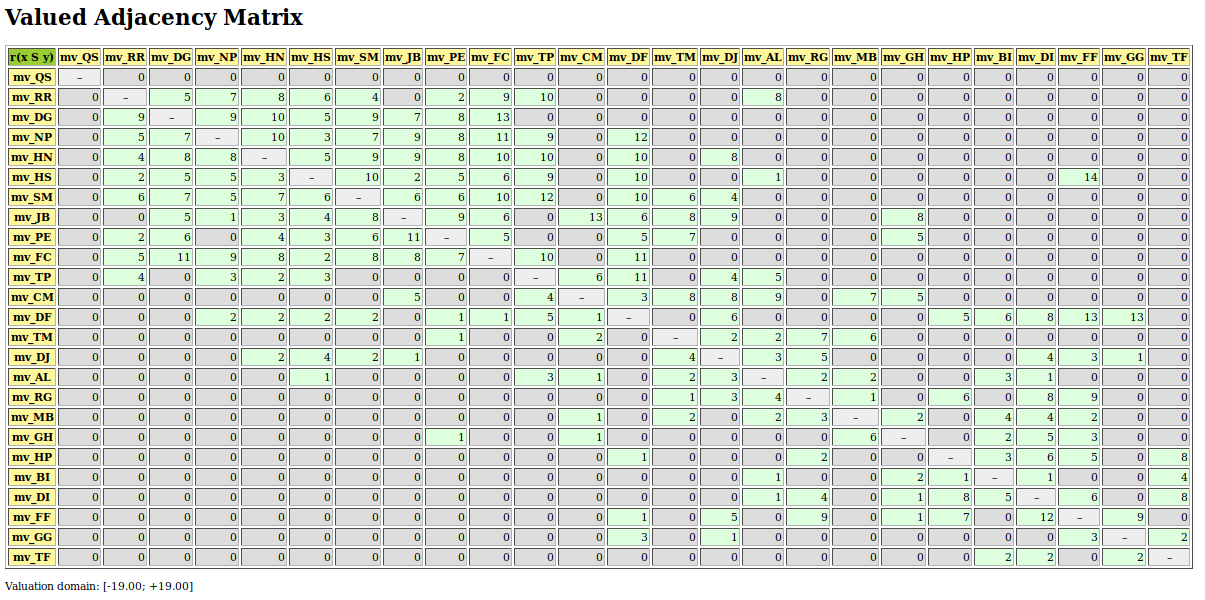
\includegraphics[width=12cm]{Figures/16-6-symmetricPart.png}
\caption{Symmetric part of \emph{graffiti07} digraph}
\label{fig:16.6}       % Give a unique label
\end{figure}

Such a preordering of the movies may, for instance, be computed with the \texttt{compute\-RankingByChoosing()} method\index{computeRankingByChoosing@\texttt{computeRankingByChoosing()}}, where we iteratively extract dominant kernels --best remaining choices-- and absorbent kernels --worst remaining choices-- (see the next Chapter). We operate therefore on the asymmetric ``\emph{better rated than}'' opinions, i.e. the codual of the ``\emph{at least as well rated as}'' opinions \footnote{A kernel in a digraph $g$ is a clique in the dual digraph $-g$.} (see Line 2 in List.~\vref{list:16.11}).
\begin{lstlisting}[caption={Bipolar ranking-by-choosing the Grafitti movies},label=list:16.11]
>>> from transitiveDigraphs import RankingByChoosingDigraph
>>> rbc = RankingByChoosingDigraph(bod,CoDual=True)
>>> rbc.showRankingByChoosing()
  Ranking by Choosing and Rejecting
    1st Best Choice ['mv_QS']
      2nd Best Choice ['mv_DG','mv_FC','mv_HN','mv_HS','mv_NP',
                       'mv_PE','mv_RR','mv_SM']
	3rd Best Choice ['mv_CM','mv_JB','mv_TM']
          4th Best Choice ['mv_AL','mv_TP']
          4th Worst Choice ['mv_AL','mv_TP']
        3rd Worst Choice ['mv_GH','mv_MB','mv_RG']
      2nd Worst Choice ['mv_DF','mv_DJ','mv_FF','mv_GG']
    1st Worst Choice ['mv_BI','mv_DI','mv_HP','mv_TF']
\end{lstlisting}

In the next Chapter~\vref{sec:17}, we thouroughly discuss the computation of such kernels in bipolar-valued digraphs.

%%%%%%% The chapter bibliography
%\normallatexbib
\clearpage
%\phantomsection
%\addcontentsline{toc}{section}{Chapter Bibliography}
\bibliographystyle{spbasic}
%\typeout{}
\bibliography{03-backMatters/reference}
%\chapter{On measuring the fitness of a multiple criteria ranking}
\label{sec:16}

\abstract*{ Starting from a motivating decision problem about how to list, from the best to the worst, a set movies that are star-rated by journalists and movie critics, the chapter shows that \Kendall 's ordinal correlation index tau may be extended to a relational bipolar-valued equivalence measure of  bipolar-valued digraphs. This finding gives way, on the one hand, to measure the fitness and fairness of multiple criteria ranking rules. On the other hand, it provides a tool for illustrating preference divergences between decision objectives and criteria.}

\abstract{ Starting from a motivating decision problem about how to list, from the best to the worst, a set movies that are star-rated by journalists and movie critics, the chapter shows that \Kendall 's ordinal correlation index tau may be extended to a relational bipolar-valued equivalence measure of  bipolar-valued digraphs. This finding gives way, on the one hand, to measure the fitness and fairness of multiple criteria ranking rules. On the other hand, it provides a tool for illustrating preference divergences between decision objectives and criteria.}

\section{Listing movies from best star-rated to worst}
\label{sec:16.1}

In a stubborn keeping with a two-valued logic, where every argument can only be true or false, there is no place for efficiently taking into account missing data or logical indeterminateness. These cases are seen as problematic and, at best are simply ignored. Worst, in modern data science, missing data get often replaced with \emph{fictive} values, potentially falsifying hence all subsequent computations.

In social choice problems, voting abstentions are, however, frequently observed and represent a social expression that may be significant for revealing non represented social preferences. And, in marketing studies, interviewees will not always respond to all the submitted questions. Again, such abstentions do sometimes contain nevertheless valid information concerning consumer preferences.

Such a case is given with  a list of star-rated movies that could be seen in town in September 2003 (source: \emph{Graffiti Star wars}, Edition Revue Luxembourg, September 2007, p. 30.). The underlying performance tableau data, stored in a file named \texttt{graffiti07.py}\footnote{to be found in the \texttt{examples} directory of the \Digraph resources}, is shown below with the \texttt{showHTMLPerformance\-Tableau()} method\index{showHTMLPerformanceTableau@\texttt{showHTMLPerformanceTableau()}}  : 
\begin{lstlisting}
>>> from outrankingDigraphs import\
...                        PerformanceTableau 
>>> gt07 = PerformanceTableau('graffiti07')
>>> gt07.showHTMLPerformanceTableau(\
...               title='Graffiti Star wars',\
...               ndigits=0)
\end{lstlisting}
\begin{figure}[h]
%\sidecaption
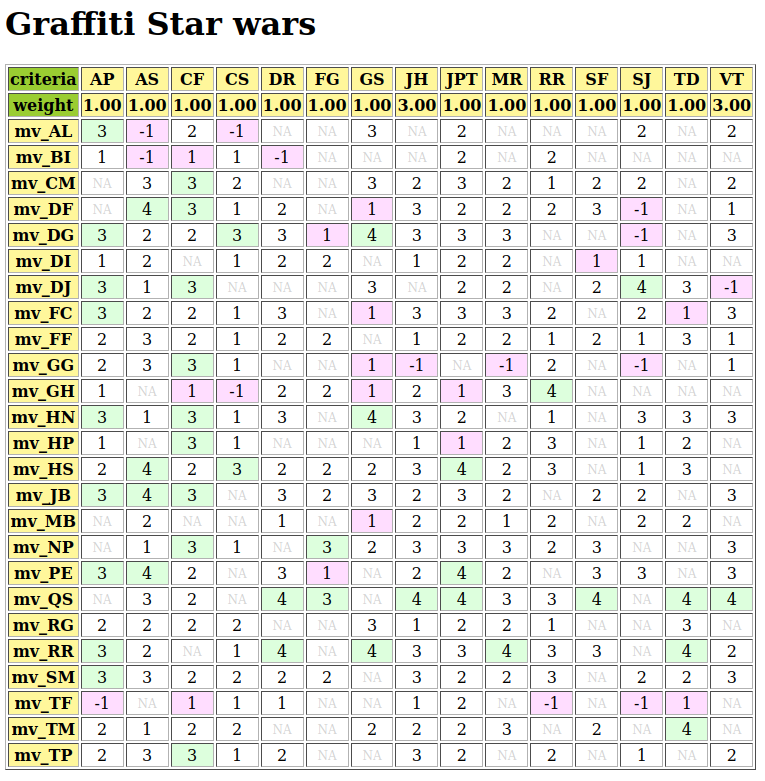
\includegraphics[width=11cm]{Figures/16-1-graffiti07_1.png}
\caption{\emph{Graffiti} magazine's movie ratings from September 2007}
\label{fig:16.1}       % Give a unique label
\end{figure}

Figure~\vref{fig:16.1} shows the star-ratings of $25$ movies by $15$ journalists and movie critics: $5$ stars (\emph{masterpiece}), $4$ stars (\emph{must be seen}), $3$ stars (\emph{excellent}), $2$ stars (\emph{good}), $1$ star (\emph{could be seen}), $-1$ star (\emph{I do not like}), $-2$ stars (\emph{I hate}), \texttt{NA} (\emph{not seen}). Notice in the second row the higher significance ($3.00$) that is granted to two locally renowned movie critics, namely \texttt{JH} and \texttt{VT}. Their opinion counts for three times the opinion of the other critics. With six times a 4 stars (\emph{must be seen}) grade, \texttt{mv\_QS} is best-rated, followed by \texttt{mv\_RR} with four times a 4 stars mark. Fewest stars obtains movie \texttt{mv\_TF} with three times a $-1$ star (\emph{don't like}) mark and five times a $1$ star mark. Notice that many movies, like movie \texttt{mv\_BI}, are only rated by some of the critics. 

To aggregate all the critics' star-ratings, the \emph{Graffiti} magazine computes for each movie a global score --the average weighted number of stars it obtained-- just ignoring the \emph{not seen} movies. Listing~\vref{list:16.1} illustrates below how to compute these global scores using the data stored in the \texttt{gt07} performance tableau. Attribute \texttt{gt07.actions}, resp. \texttt{gt07.criteria}, contains the description of the 25 movies, resp. the 15 critics. The actual star-ratings are to be found in the \texttt{gt07.evaluation} attribute.
\begin{lstlisting}[caption={Computing the average weighted number of stars per movie},label=list:16.1,basicstyle=\ttfamily\scriptsize]
>>> # gt07 = PerformanceTableau('graffiti07')
>>> globalScores = {}
>>> for mv in gt07.actions:
>>>     globalScores[mv] = Decimal('0')
>>>     sumWeights = Decimal('0')
>>>     for critic in gt07.criteria:
>>>         stars = gt07.evaluation[critic][mv]
>>>         if stars != gt07.NA:
>>>             weight = gt07.criteria[critic]['weight']
>>>             globalScores[mv] += (stars * weight)
>>>             sumWeights += weight
>>>     globalScores[mv] /= sumWeights
>>> graffitiList = [(globalScores[mv],mv) for mv in globalScores]
>>> graffitiList.sort(reverse=True)
>>> for item in graffitiList:
>>>     print('%s: %.2f' % (item[1],item[0]) )
  mv_QS: 3.60
  mv_RR: 2.88
  mv_PE: 2.67
  mv_JB: 2.62
  mv_HN: 2.62
  mv_NP: 2.60
  mv_HS: 2.60
  mv_DG: 2.56
  mv_SM: 2.53
  mv_FC: 2.41
  mv_TP: 2.21
  mv_CM: 2.20
  mv_TM: 2.17
  mv_DF: 1.94
  mv_RG: 1.83
  mv_MB: 1.73
  mv_GH: 1.67
  mv_DJ: 1.67
  mv_FF: 1.61
  mv_AL: 1.60
  mv_HP: 1.55
  mv_DI: 1.42
  mv_GG: 0.71
  mv_BI: 0.71
  mv_TF: 0.55
\end{lstlisting}

The global scrores ranking confirms in Lines 17-18 both leading movies --\texttt{mv\_QS} ($3.60$) and \texttt{mv\_RR} ($2.88$) -- as well as in Line 41 the weakest rated one --\texttt{mv\_TF} ($0.55$). Mind however that these global averages, due to the numerous missing grades, are not computed with commensurable denominators; some critics do indeed use a more or less extended range of stars. The movies not seen for instance by critic \texttt{SJ} are favoured, as this critic is severer than others in her rating. Dropping the movies that were not graded by all the critics is not possible either, as none of the $25$ movies was actually rated by all the $15$ critics. Providing a fictive value for the many not seen situations, will as well always somehow falsify the global scores. What to do?

A better approach is to rank the movies on the basis of pairwise bipolar-valued  ``\emph{rated at least as well as}'' statements. Under this epistemic argumentation approach, missing grades are naturally treated as opinion abstentions and hence do not falsify the logical computations. Such a \NetFlows ranking from best-rated to weakest-rated is provided by the \textbf{heatmap} browser view generated with the \texttt{showHTMLPerformanceHeatmap()} method\index{showHTMLPerformanceHeatmap@\texttt{showHTMLPerformanceHeatmap()}} (see List.~\vref{list:16.2}).
\begin{lstlisting}[caption={Showing the movie from best to worst rated in a heatmap view},label=list:16.2]
>>> gt07.showHTMLPerformanceHeatmap(\
...            pageTitle='Ranking the movies',\  
...            rankingRule='NetFlows',
...            Correlations=True,\
...            ndigits=0)
\end{lstlisting}
\begin{figure}[h]
%\sidecaption
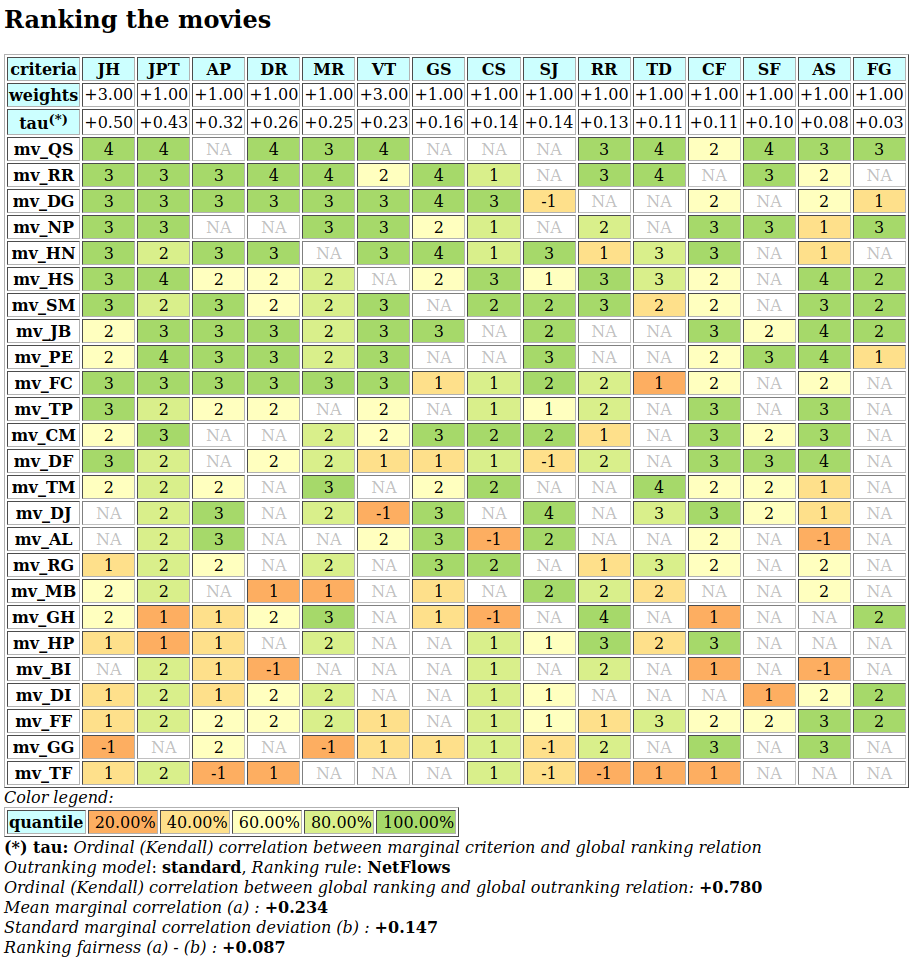
\includegraphics[width=11cm]{Figures/16-2-graffiti07_2.png}
\caption{\emph{Graffiti} magazine's movie ratings from September 2007 ranked with the \NetFlows rule}
\label{fig:16.2}       % Give a unique label
\end{figure}

The \NetFlows ranking shown in Fig.~\vref{fig:16.2} confirms again that movie \texttt{mv\_QS}, with $6$ \emph{must be seen} marks, is correctly best-ranked and the movie \texttt{mv\_TF} is worst-ranked with five \emph{don't like} marks. 

It is fair, however, to eventually mention here that the \emph{Graffiti} magazine's average stars ranking rule is actually showing a very similar result. Indeed, average scores usually confirm well all evident pairwise comparisons, yet \emph{enforce} comparability for all less evident ones. How to judge now the fitness of a given ranking rule?

This is the purpose of the ordinal correlation \emph{tau} indexes shown in Fig.~\vref{fig:16.2} 3rd row. Computing these ordinal correlation indexes is the subject of the next Section.
 
\section{\Kendall 's ordinal correlation tau index}
\label{sec:16:2}

M. G. Kendall\index{Kendall@\emph{Kendall M.G.}} defined his ordinal correlation $\tau$ (\emph{tau}) index for linear orders of dimension $n$ as a balancing of the number $Co$ of correctly oriented pairs against the number $In$ of incorrectly oriented pairs \citep{KEN-1938}. The total number of irreflexive pairs being $n(n-1)$, in the case of linear orders, $Co + In \;=\; n(n-1)$.  Hence $\tau \;=\; \big(\frac{Co}{n(n-1)}\big) \,-\, \big(\frac{In}{n(n-1)}\big)$. In case $In$ is zero, $\tau \;=\; +1$  (all pairs are equivalently oriented); inversely, in case $Co$ is zero, $\tau \;=\; -1$ (all pairs are differently oriented).

Noticing that $\frac{Co}{n(n-1)} \;=\; 1 \,-\, \frac{In}{n(n-1)}$, and recalling that the bipolar-valued negation is operated by changing the sign of the characteristic value:
\begin{equation}
      \tau \;=\; 1 -2\frac{In}{n(n-1)} \;=\; -\big(\,2\frac{In}{n(n-1)} \,-\, 1\,\big) \;=\; 2\frac{Co}{n(n-1)} \,-\, 1,
\end{equation} 
\Kendall 's original \emph{tau} definition implemented in fact the bipolar-valued negation of the non equivalence of two linear orders, i.e. the normalized majority margin of equivalently oriented irreflexive pairs.

Let \texttt{r1} and \texttt{r2} be two random crisp relations defined on a same set of 5 alternatives. We may compute \Kendall 's \emph{tau} index as shown in List.~\vref{list:16.3}.
\begin{lstlisting}[caption={Computing a relational equivalence digraph},label=list:16.3]
>>> from randomDigraphs import RandomDigraph
>>> r1 = RandomDigraph(order=5,Bipolar=True)
>>> r2 = RandomDigraph(order=5,Bipolar=True)
>>> from digraphs import EquivalenceDigraph
>>> eqd = EquivalenceDigraph(r1,r2)
>>> eqd.showRelationTable(ReflexiveTerms=False)
  * ---- Relation Table -----
  r(<=>)|  'a1'	  'a2'	  'a3'	  'a4'	  'a5'	  
  ------|-------------------------------------
   'a1' |    -   -1.00   1.00   -1.00    1.00	 
   'a2' |  -1.00   -    -1.00    1.00   -1.00	 
   'a3' |  -1.00 -1.00    -      1.00    1.00	 
   'a4' |  -1.00  1.00  -1.00     -      1.00	 
   'a5' |  -1.00  1.00  -1.00    1.00     - 	 
   Valuation domain: [-1.00;1.00]
>>> eqd.correlation
  {'correlation': -0.1, 'determination': 1.0}
\end{lstlisting}
In the table of the equivalence relation $(\mathtt{r1}\, \Leftrightarrow\, \mathtt{r2})$ above (see List.~\vref{list:16.1} Lines 10-14), we observe that the normalized majority margin of equivalent versus non equivalent irreflexive pairs amounts to $(9 - 11)/20 = -0.1$, i.e. the value of \Kendall 's \emph{tau} index in this plainly determined crisp case (see Line 17).

What happens now with more or less determined and even partially indeterminate relations? May we proceed in a similar way?

\section{Bipolar-valued relational equivalence}
\label{sec:16.3}

Two random bipolar-valued digraphs \texttt{d1} and \texttt{d2} of order five, generated in List.~\vref{list:16.4}, will help exploring this idea.
\begin{lstlisting}[caption={Two random bipolar-valued digraphs},label=list:16.4]
>>> from randomDigraphs import RandomValuationDigraph
>>> d1 = RandomValuationDigraph(order=5,seed=1)
>>> d1.showRelationTable(ReflexiveTerms=False)
  * ---- Relation Table -----
   r(d1)|   'a1'   'a2'   'a3'   'a4'   'a5'	  
  ------|------------------------------------
   'a1' |    - 	  -0.66	  0.44	  0.94	-0.84	 
   'a2' |  -0.36    - 	 -0.70	  0.26	 0.94	 
   'a3' |   0.14   0.20	   - 	  0.66	-0.04	 
   'a4' |  -0.48 - 0.76	  0.24	   -  	-0.94	 
   'a5' |  -0.02   0.10	  0.54	  0.94    - 	 
   Valuation domain: [-1.00;1.00]
>>> d2 = RandomValuationDigraph(order=5,seed=2)
>>> d2.showRelationTable(ReflexiveTerms=False)
  * ---- Relation Table -----
   r(d2)|   'a1'   'a2'   'a3'   'a4'   'a5'	  
  ------|-----------------------------------
   'a1' |   -     -0.86  -0.78  -0.80  -0.08	 
   'a2' |  -0.58    -     0.88   0.70  -0.22	 
   'a3' |  -0.36   0.54    -    -0.46   0.54	 
   'a4' |  -0.92   0.48   0.74    -    -0.60	 
   'a5' |   0.10   0.62   0.00   0.84    - 	 
   Valuation domain: [-1.00;1.00]
\end{lstlisting}
In the generated random digraphs \texttt{d1} and \texttt{d2}, 9 pairs, like \texttt{(a1,a2)} or \texttt{(a3,a2)} for instance, appear equivalently oriented (see Lines 7,18 or 9,20). The \texttt{Equiva\-lenceDigraph} class\index{EquivalenceDigraph@\texttt{EquivalenceDigraph} class} computes this bipolar-valued relational equivalence between digraphs \texttt{d1} and \texttt{d2} (see List.~\vref{list:16.5}).
\begin{lstlisting}[caption={Bipolar-valued Equivalence Digraph},label=list:16.5]
>>> from digraphs import EquivalenceDigraph
>>> eqd = EquivalenceDigraph(d1,d2)
>>> eqd.showRelationTable(ReflexiveTerms=False)
  * ---- Relation Table -----
   r(<=>)|  'a1'  'a2'   'a3'   'a4'   'a5'	  
   ------|---------------------------------
   'a1' |   - 	  0.66  -0.44  -0.80   0.08	 
    'a2' |  0.36   -    -0.70   0.26  -0.22	 
    'a3' | -0.14  0.20    -    -0.46  -0.04	 
    'a4' |  0.48 -0.48   0.24    -     0.60	 
    'a5' | -0.02  0.10   0.00   0.84    - 	 
   Valuation domain: [-1.00;1.00]
\end{lstlisting}

In our bipolar-valued epistemic logic, logical disjunctions and conjunctions are implemented as $\max$, respectively $\min$ operations. Notice also that the logical equivalence $(\mathtt{d1}\, \Leftrightarrow\, \mathtt{d2})$ corresponds to a double implication $(\mathtt{d1}\, \Rightarrow\, \mathtt{d2})\; \wedge \; (\mathtt{d2}\, \Rightarrow\,  \mathtt{d1})$ and that the implication $(\mathtt{d1} \Rightarrow \mathtt{d2})$ is logically equivalent to the disjunction $(\neg \mathtt{d1} \vee \mathtt{d2})$.

When $r(x\,\mathtt{d1}\, y)$ and $r(x\,\mathtt{d2}\; y)$ denote the bipolar-valued characteristic values of relation \texttt{d1}, resp. \texttt{d2}, we may hence compute as follows a majority margin $M(\mathtt{d1} \Leftrightarrow \mathtt{d2})$ between equivalently and not equivalently oriented irreflexive pairs $(x,y)$:
\begin{equation}\label{eq:16:2}
  \begin{split}
&M(\mathtt{d1} \Leftrightarrow \mathtt{d2}) \; =\\
&\quad \quad \sum_{(x \neq y)} \Big[ \min \Big( \max \big( -r(x \,\mathtt{d1}\, y), r(x \,\mathtt{d2}\, y)\big), \max \big( -r(x \,\mathtt{d2}\, y), r(x \,\mathtt{d1}\, y)\big) \Big) \Big]\;.
\end{split}
\end{equation}

$M(\mathtt{d1} \Leftrightarrow \mathtt{d2})$ is thus given by the sum of the non reflexive terms of the relation table of $eqd$, the relational equivalence digraph computed above (see List.~\vref{list:16.5}). In the crisp case, $M(\mathtt{d1}\,\Leftrightarrow\, \mathtt{d2})$  is normalized with the maximum number of possible irreflexive pairs, namely $n(n-1)$. In the extended $r$-valued case, the maximal possible equivalence majority margin $M$ corresponds to the sum $D$ of the conjoint determinations of $(x \,\mathtt{d1}\, y)$ and $(x \,d2\, y)$ (see \citet{BIS-2012a}):
\begin{equation}
  D \;=\; \sum_{x \neq y} \min \Big[ abs\big(r(x \,\mathtt{d1}\, y) \big), abs \big( r(x \,\mathtt{d2}\, y \big)  \Big]\;,
\end{equation}
and we obtain hence in the general $r$ -valued case:
\begin{equation}\label{eq:16.4}
  \tau(\mathtt{d1},\mathtt{d2}) \;=\; \frac{M(\mathtt{d1}\,\Leftrightarrow\, \mathtt{d2})}{D}\;.
\end{equation}

$\tau(\mathtt{d1},\mathtt{d2})$ corresponds so to the classical ordinal correlation index, yet restricted to the conjointly determined parts of the given digraphs $\mathtt{d1}$ and $\mathtt{d2}$. In the limit case of two crisp linear orders, $D$ equals $n(n-1)$, i.e. the number of irreflexive pairs, and we recover \Kendall 's original \emph{tau} index definition.

It is worthwhile noticing that the ordinal correlation index $\tau(\mathtt{d1},\mathtt{d2})$ one obtains above corresponds in fact to the ratio of:
\begin{itemize}
\item $r(\mathtt{d1}\,\Leftrightarrow\, \mathtt{d2}) \;=\; \frac{M(\mathtt{d1}\,\Leftrightarrow\, \mathtt{d2})}{n(n-1)}$:\\the normalized majority margin of the pairwise \emph{relational} equivalence statements, also called \emph{valued ordinal correlation}, and 
\item $d \;=\; \frac{D}{n(n-1)}$:\\ the normalized determination of the corresponding pairwise relational equivalence statements, in fact the \emph{determinateness} of the relational equivalence digraph.
\end{itemize}

The epistemic determination effect is thus successfully \emph{out-factored} from the ordinal correlation effect. With completely determined relations, $\tau(\mathtt{d1},\mathtt{d2}) \;=\; r(\mathtt{d1}\,\Leftrightarrow\, \mathtt{d2})$. The ordinal correlation with a completely indeterminate digraph, i.e. when $D = 0$, is set by convention to the indeterminate correlation value $0.0$. With uniformly chosen random $r$-valued digraphs, the expected $\tau$ index is $0.0$, denoting in fact an indeterminate relational equivalence. The corresponding expected normalized determination $d$ is about $0.333$ (see \citep{BIS-2012a}).

We may below verify Eq.~\vref{eq:6.4} with help of the equivalence digraph $eqd$ computed in List.~\vref{list:16.5}.
\begin{lstlisting}[caption={Computing the ordinal correlation index from the equivalence digraph},label=list:16.6]
>>> # eqd = EquivalenceDigraph(d1,d2)
>>> M = Decimal('0'); D = Decimal('0')
>>> n2 = eqd.order*(eqd.order - 1)
>>> for x in eqd.actions:
...     for y in eqd.actions:
...         M += eqd.relation[x][y]
...         D += abs(eqd.relation[x][y])
>>> print('r(rd1<=>rd2) = %+.3f, d = %.3f, tau = %+.3f' %\
          (M/n2,D/n2,M/D))   
  r(rd1<=>rd2) = +0.026, d = 0.356, tau = +0.073  
\end{lstlisting}

The \Digraph resources directly provide for the preceding computations the \texttt{compute\-OrdinalCorrelation()} method\index{computeOrdinalCorrelation@\texttt{computeOrdinalCorrelation()}} which renders a dictionary with a \texttt{correlation} ($\tau$) and a \texttt{determina\-tion} ($d$) attribute. We may recover $r(d1\,\Leftrightarrow\, d2)$ by multiplying $\tau$ with $d$ (see List.~\vref{list:16.7} Line 4). 
\begin{lstlisting}[caption={Computing the valued ordinal correlation index},label=list:16.7]
>>> corrd1d2 = d1.computeOrdinalCorrelation(d2)
>>> tau = corrd1d2['correlation']
>>> d = corrd1d2['determination']
>>> r = tau * d
>>> print('tau(d1,d2) = %+.3f, d = %.3f,\
...        r(d1<=>d2) = %+.3f' % (tau, d, r))
  tau(d1,d2) = +0.073, d = 0.356, r(d1<=>d2) = +0.026
\end{lstlisting}

The \Digraph resources provide for convenience a direct \texttt{showCorrela\-tion()} method\index{showCorrelation@\texttt{showCorrelation()}}:
\begin{lstlisting}
>>> d1.showCorrelation(\
...       d1.computeOrdinalCorrelation(d2) )
  Correlation indexes:
    Extended Kendall tau       : +0.073
    Epistemic determination    :  0.356
    Bipolar-valued equivalence : +0.026
\end{lstlisting}

We are now ready for assessing the quality of the \NetFlows ranking of the movies shown in the heat map view of Fig.~\vref{fig:16.2}. 

\section{Fitness of ranking heuristics}
\label{sec:16.3}

The \NetFlows ranking of the movies shown in the heatmap view in Fig.~\vref{fig:16.2} is based on the bipolar-valued outranking digraph modelling the pairwise global ``\emph{rated at least as well as}'' relation among the $25$ movies from the performance tableau instance \texttt{gt07}.
\begin{lstlisting}[caption={The bipolar-valued outranking digraph of the star-rated movies},label=list:16.8]
>>> bod = BipolarOutrankingDigraph(gt07)
  *------- Object instance description ------*
   Instance class   : BipolarOutrankingDigraph
   Instance name    : rel_grafittiPerfTab.xml
   Actions          : 25
   Criteria         : 15
   Size             : 390
   Determinateness  : 65%
   Valuation domain : {'min': Decimal('-1.0'),
                       'med': Decimal('0.0'),
                       'max': Decimal('1.0'),}
>>> g.computeCoSize()
  188
\end{lstlisting}
Listing~\vref{list:16.8} reveals that the outranking digraph \texttt{bod} contains $390$ positively validated (Line 7), $188$ positively invalidated (Line 13)\index{computeCoSize@\texttt{computeCoSize()}}, and 22 indeterminate outranking situations from the potential $25 \times 24 = 600$ irreflexive movie pairs.

Listing~\vref{list:16.9} illustrates with the \texttt{NetFlowsOrder} class \index{NetFlowsOrder@\texttt{NetFlowsOrder} class} from the \texttt{linearOr\-ders} module\index{linearOrders@\texttt{linearOrders} module} how to compute the global \NetFlows ranking \texttt{nf}, as shown in the ordered heat map of Fig.~\vref{fig:16.2} and the bipolar-valued relational equivalence of the \texttt{nf} ranking with each one the individual critic's star-ratings.
\begin{lstlisting}[caption={Computing marginal criterion correlations with global \NetFlows ranking},label=list:16.9]
>>> from linearOrders import NetFlowsOrder
>>> nf = NetFlowsOrder(bod)
>>> nf.netFlowsRanking
  ['mv_QS', 'mv_RR', 'mv_DG', 'mv_NP', 'mv_HN', 'mv_HS', 'mv_SM',
   'mv_JB', 'mv_PE', 'mv_FC', 'mv_TP', 'mv_CM', 'mv_DF', 'mv_TM',
   'mv_DJ', 'mv_AL', 'mv_RG', 'mv_MB', 'mv_GH', 'mv_HP', 'mv_BI',
   'mv_DI', 'mv_FF', 'mv_GG', 'mv_TF']
>>> for i,item in enumerate(\
...       bod.computeMarginalVersusGlobalRankingCorrelations(\
...              nf.netFlowsRanking,ValuedCorrelation=True) ):\
...     print('r(%s<=>nf) = %+.3f' % (item[1],item[0]) )   

  r(JH<=>nf)  = +0.500
  r(JPT<=>nf) = +0.430
  r(AP<=>nf)  = +0.323
  r(DR<=>nf)  = +0.263
  r(MR<=>nf)  = +0.247
  r(VT<=>nf)  = +0.227
  r(GS<=>nf)  = +0.160
  r(CS<=>nf)  = +0.140
  r(SJ<=>nf)  = +0.137
  r(RR<=>nf)  = +0.133
  r(TD<=>nf)  = +0.110
  r(CF<=>nf)  = +0.110
  r(SF<=>nf)  = +0.103
  r(AS<=>nf)  = +0.080
  r(FG<=>nf)  = +0.027
\end{lstlisting}

In List.~\vref{list:16.9} (see Lines 13-27), we obtain the relational equivalence characteristic values shown in the third row of the ranked heatmap (see Fig.~\vref{fig:16.2}). The global \NetFlows ranking \texttt{nf} represents obviously a rather balanced compromise with respect to each movie critic's star-ratings, as there appears no negative correlation with anyone of them. The ranking \texttt{nf} apparently takes also correctly in account that the journalist $JH$, a locally renowned movie critic, shows a higher significance weight (see Line 13).

The ordinal correlation between the global \NetFlows ranking and the outranking digraph \texttt{bod} may be furthermore computed as illstrated in List.~\vref{list:16.10}: 
\begin{lstlisting}[caption={Computing the ordinal correlation between \NetFlows and global outranking digraph},label=list:16.10]
>>> corrgnf = bod.computeOrdinalCorrelation(nf)
>>> bod.showCorrelation(corrgnf)
  Correlation indexes:
    Extended Kendall tau       : +0.780
    Epistemic determination    :  0.300
    Bipolar-valued equivalence : +0.234
\end{lstlisting}
One may notice in Line 4 that the ordinal correlation $\tau(\mathtt{bod},\mathtt{nf})$ index between the \NetFlows ranking $\mathtt{nf}$ and the determined part of the outranking digraph $\mathtt{bod}$ is quite high ($+0.78$). Due to the rather high number of missing data, the $r$ -valued relational equivalence between the $\mathtt{nf}$ and the $\mathtt{bod}$ digraph, with a characteristics value of only $+0.234$, may be misleading. Yet, $+0.234$ still corresponds to a $62\%$ majority support of the movie critics' star-ratings.

It would be interesting to compare similarly the correlations one may obtain with other global ranking heuristics, like the \Copeland ranking rule.

\section{Illustrating preference divergences}
\label{sec:16.4}

The bipolar-valued relational equivalence indexes gives us, via the \texttt{showCrite\-riaCorrelationTable(ValuedCorrelation=True)} method\index{showCriteriaCorrelationTable@\texttt{showCriteriaCorrelationTable()}}, a further measure for studying how \emph{divergent} may appear the rating opinions expressed by the movie critics. 
\begin{figure}[h]
%\sidecaption
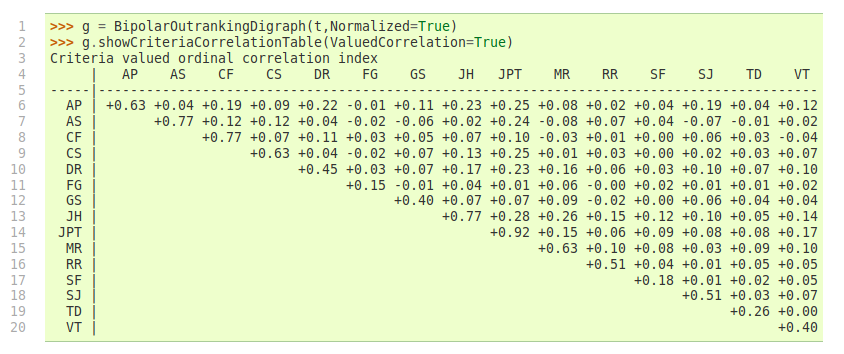
\includegraphics[width=12cm]{Figures/16-3-correlationTable.png}
\caption{Pairwise valued correlation of movie critics.} 
\label{fig:16.3}       % Give a unique label
\end{figure}

It is remarkable to notice in Fig.~\vref{fig:16.3} that, due to the quite numerous missing data, all pairwise valued ordinal correlation indexes $r(x\Leftrightarrow y)$ appear to be of low value, except the diagonal ones. These reflexive indexes $r(x\Leftrightarrow x)$ would trivially all amount to $+1.0$ in a plainly determined case. Here they indicate a reflexive normalized determination score $d$, i.e. the proportion of pairs of movies each critic did evaluate. Critic \texttt{JPT} (the editor of the Graffiti magazine), for instance, evaluated all but one ($d = 24\times23/600 = 0.92$), whereas critic \texttt{FG} evaluated only 10 movies among the 25 in discussion ($d = 10\times9/600 = 0.15$).

To get a picture of the actual divergence of rating opinions concerning jointly seen pairs of movies, we may develop a Principal Component Analysis of the corresponding $\tau$ correlation matrix\footnote{The 3D PCA plot method requires a running R statistics software  (https://www.r-project.org/) installation and the Calmat matrix calculator (see the \texttt{calmat} directory in the \Digraph resources)}. The 3D plot of the first 3 principal axes is shown in Fig.~\vref{fig:16.2}.\index{export3DplotOfCriteriaCorrelation@\texttt{export3DplotOfCriteriaCorrelation()}}
\begin{lstlisting}
>>> bod.export3DplotOfCriteriaCorrelation(\
...                     ValuedCorrelation=False)
\end{lstlisting}
\begin{figure}[h]
%\sidecaption
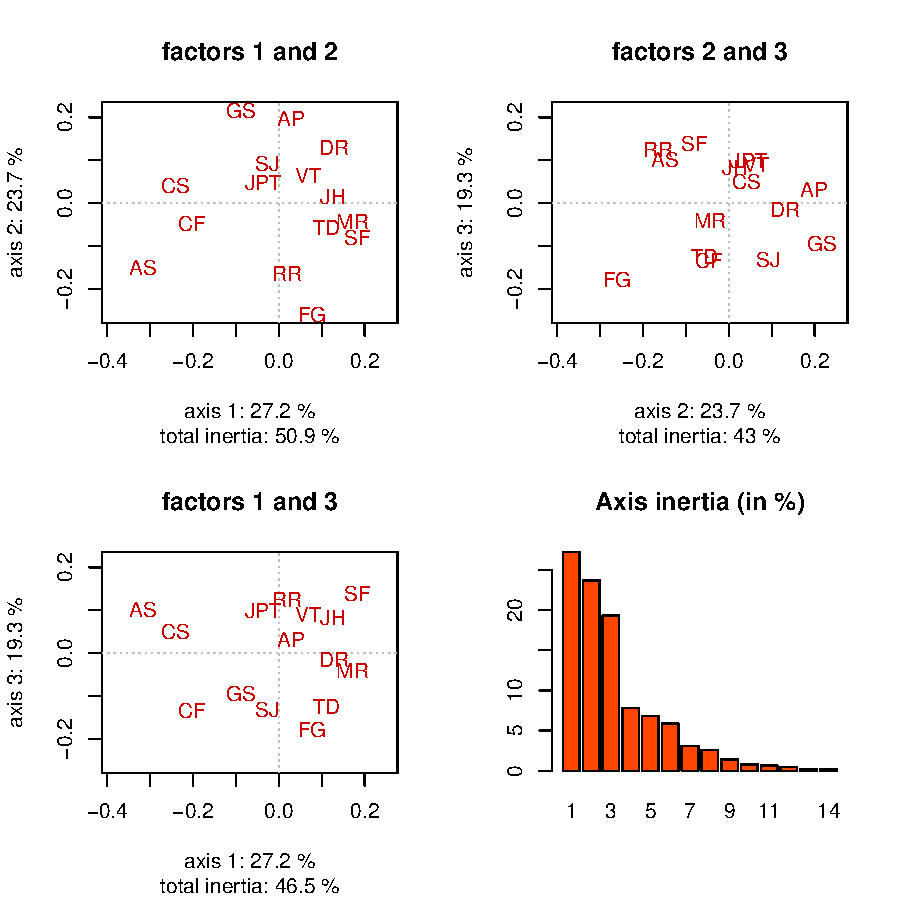
\includegraphics[width=10cm]{Figures/16-4-correlationPCA.pdf}
\caption{3D PCA plot of the criteria ordinal correlation matrix.}
\label{fig:16.4}       % Give a unique label
\end{figure}
The first 3 principal axes support together about $70\%$ of the total inertia. Most eccentric and opposed in their respective rating opinions appear, on the first principal axis with $27.2\%$ inertia, the conservative daily press against labour and public press. On the second principal axis with $23.7.7\%$ inertia, it is the people press versus the cultural critical press. And, on the third axis with still $19.3\%$ inertia, the written media appear most opposed to the radio media.

\section{Exploring the ``\emph{better rated}''  and the ``\emph{as well as rated}'' opinions}
\label{sec:16.5}

In order to furthermore study the quality of a ranking result, it may be interesting to have a separate view on the asymmetric and symmetric parts of the ``\emph{at least as well rated as}'' opinions (see Section \vref{sec:2.3}).

Let us first inspect the pairwise asymmetric part, namely the ``\emph{better rated than}'' and ``\emph{less well rated than}'' opinions of the movie critics. \index{AsymmetricPartialDigraph@\texttt{AsymmetricPartialDigraph} class}
\begin{lstlisting}
>>> from digraphs import AsymmetricPartialDigraph
>>> ag = AsymmetricPartialDigraph(bod)
>>> ag.showHTMLRelationTable(\
...    actionsList=g.computeNetFlowsRanking(),ndigits=0)
\end{lstlisting}
\begin{figure}[h]
%\sidecaption
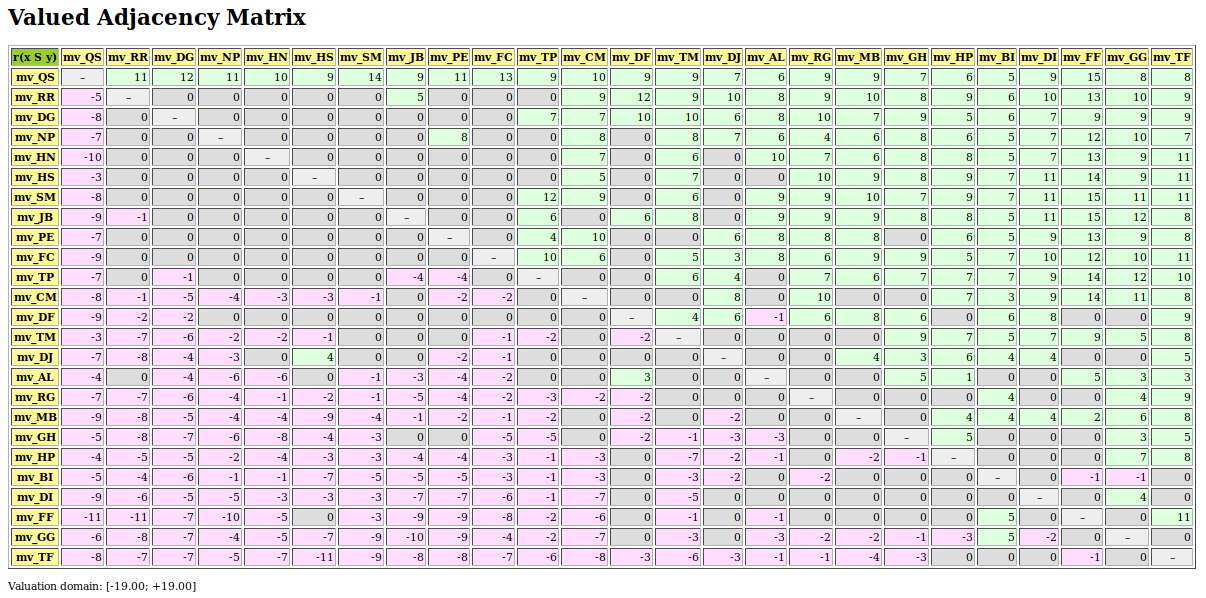
\includegraphics[width=12cm]{Figures/16-5-asymmetricPart.png}
\caption{Asymmetric part of \emph{graffiti07} digraph}
\label{fig:16.5}       % Give a unique label
\end{figure}

We notice in Fig.~\vref{fig:16.5} that the \NetFlows ranking rule inverts in fact just three ``\emph{less well rated than}'' opinions and four ``\emph{better rated than}'' ones. A similar look in Fig.~\vref{fig:16.6} at the symmetric part --the pairwise ``\emph{as well rated as}'' opinions-- suggests a preordered preference structure in several equivalently rated classes. \index{SymmetricPartialDigraph@\texttt{SymmetricPartialDigraph} class}
\begin{lstlisting}
>>> from digraphs import SymmetricPartialDigraph
>>> sg = SymmetricPartialDigraph(bod)
>>> sg.showHTMLRelationTable(\
...          actionsList=g.computeNetFlowsRanking(),\
...          ndigits=0)
\end{lstlisting}
\begin{figure}[h]
%\sidecaption
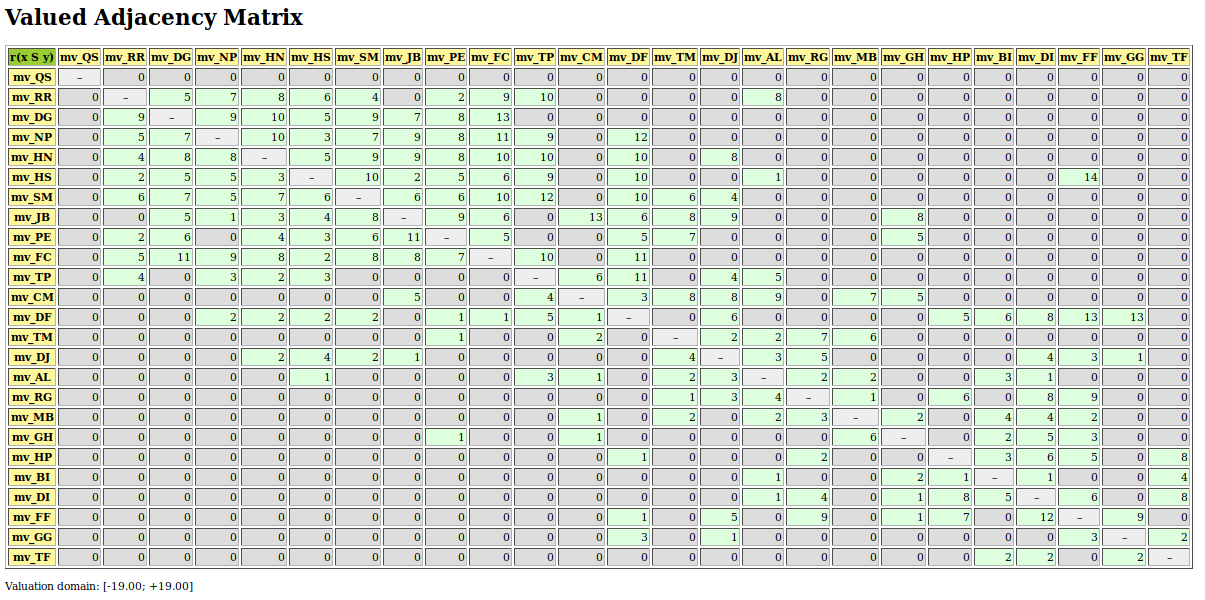
\includegraphics[width=12cm]{Figures/16-6-symmetricPart.png}
\caption{Symmetric part of \emph{graffiti07} digraph}
\label{fig:16.6}       % Give a unique label
\end{figure}

Such a preordering of the movies may, for instance, be computed with the \texttt{compute\-RankingByChoosing()} method\index{computeRankingByChoosing@\texttt{computeRankingByChoosing()}}, where we iteratively extract dominant kernels --best remaining choices-- and absorbent kernels --worst remaining choices-- (see the next Chapter). We operate therefore on the asymmetric ``\emph{better rated than}'' opinions, i.e. the codual of the ``\emph{at least as well rated as}'' opinions \footnote{A kernel in a digraph $g$ is a clique in the dual digraph $-g$.} (see Line 2 in List.~\vref{list:16.11}).
\begin{lstlisting}[caption={Bipolar ranking-by-choosing the Grafitti movies},label=list:16.11]
>>> from transitiveDigraphs import RankingByChoosingDigraph
>>> rbc = RankingByChoosingDigraph(bod,CoDual=True)
>>> rbc.showRankingByChoosing()
  Ranking by Choosing and Rejecting
    1st Best Choice ['mv_QS']
      2nd Best Choice ['mv_DG','mv_FC','mv_HN','mv_HS','mv_NP',
                       'mv_PE','mv_RR','mv_SM']
	3rd Best Choice ['mv_CM','mv_JB','mv_TM']
          4th Best Choice ['mv_AL','mv_TP']
          4th Worst Choice ['mv_AL','mv_TP']
        3rd Worst Choice ['mv_GH','mv_MB','mv_RG']
      2nd Worst Choice ['mv_DF','mv_DJ','mv_FF','mv_GG']
    1st Worst Choice ['mv_BI','mv_DI','mv_HP','mv_TF']
\end{lstlisting}

In the next Chapter~\vref{sec:17}, we thouroughly discuss the computation of such kernels in bipolar-valued digraphs.

%%%%%%% The chapter bibliography
%\normallatexbib
\clearpage
%\phantomsection
%\addcontentsline{toc}{section}{Chapter Bibliography}
\bibliographystyle{spbasic}
%\typeout{}
\bibliography{03-backMatters/reference}
%\input{02-mainMatters/16-chapterCorrelation.bbl}